% results_section.tex: GENERATED, do not edit.
% Built by scripts/paper/build_section.jl on 2026-10-05 16:39
% from section_source.tex + captions.tex + values.tex + convergence/values.tex +
% Ridge, ablation, assessment-access, and centrality values + figmeta.tex + supplement figure order;
% sweep 2026-09-05_adeaa06_nn; each input retains its own analysis provenance below.
% manuscript commit 6eda609dcad3981f3cca6fd8a7b33f3481ceb08f; uncommitted manuscript/build changes included.
% Every number was computed from the saved sweep data by the reporting scripts.
% Display: estimates at most two decimals; percentages rounded to whole points.
% Exact parameter settings retain their source precision.
% Input: output/main/values.tex; SHA256: a83b703be50b9c810bb5764d2f578cb9766063e02a4ca518e3fb72efebf36e7e
% Input commit: output/main/values.tex; analysis commit: 78aca30174ee31db965ab19cd12807a2d61d71f7
% Input: output/main/convergence/values.tex; SHA256: eb9f3bceecbaa9d30f437c39b35cd9cfc543eb808076c1fa22c334340139ff43
% Input commit: output/main/convergence/values.tex; analysis commit: 78aca30174ee31db965ab19cd12807a2d61d71f7
% Input: output/ridge/paired/analysis/paper_values.tex; SHA256: 21e2d3921aeb32305542071a72dfbb81e8e97ed5f3a7125665ff50e0d4dac3ac
% Input commit: output/ridge/paired/analysis/paper_values.tex; data analysis commit: 78aca30174ee31db965ab19cd12807a2d61d71f7
% Input commit: output/ridge/paired/analysis/paper_values.tex; nn analysis commit: 78aca30174ee31db965ab19cd12807a2d61d71f7
% Input commit: output/ridge/paired/analysis/paper_values.tex; nn-ridge comparison analysis commit: de4d915ddec550d37df54fca4da1f5ba3e0af5c1
% Input: output/ridge/ablations/analysis/paper_values.tex; SHA256: f3b1b9cc8e40d3c2c47670c30a373cb2808dc4dbca099115221e59031026d981
% Input commit: output/ridge/ablations/analysis/paper_values.tex; analysis commit: de4d915ddec550d37df54fca4da1f5ba3e0af5c1
% Input: output/assessment_access/paper_values.tex; SHA256: eff41ceea82f22da5739022d137f82c467668d995cadcb7df266f5bc7f40d6b2
% Input commit: output/assessment_access/paper_values.tex; data analysis commit: 00e3dba59efcec8d189f1b0cc99c6471abd28e6a
% Input: output/main/centrality_values.tex; SHA256: fb43517fc3bcb3e20fe20087d2c8b550253d3729a547652612dbc27c8471c781
% Input commit: output/main/centrality_values.tex; data analysis commit: de4d915ddec550d37df54fca4da1f5ba3e0af5c1
% Input: output/main/figmeta.tex; SHA256: 98f73d0f80ba17d9c46fefdb269cd15f291c018ed30d1e1296270d592d3768af
% Input commit: output/main/figmeta.tex; data analysis commit: 78aca30174ee31db965ab19cd12807a2d61d71f7
% Input commit: output/main/figmeta.tex; ridge ablation analysis commit: de4d915ddec550d37df54fca4da1f5ba3e0af5c1
% Input commit: output/main/figmeta.tex; base ridge analysis commit: 78aca30174ee31db965ab19cd12807a2d61d71f7
% Figure SHA256: figures/assessment_not_access.png 88895ca1ec59da01b64495bc2391260df122571e43900e8a3803495d6d1740a3
% Figure SHA256: figures/assessment_access_3.png 32dbff8441f0aa3fe724108f57cc59362a0511172aa5f8eb20661cb5a6653709
% Figure SHA256: figures/information_sources_net_output_channels.png 7b4e475a67c45e39830dbc8e5653ef6e64b6bef43ad0c213b15e11439b6fd292
% Figure SHA256: figures/centrality_and_assessment.png 09de2c59b045cf22954e7ec79b6fe0b29cfd49974dc9ffbfcfd91babf42896f6
% Source fingerprint: 33c615202538bd04791992905c5186fa8149dd5a6916b5369ab09e34d771145f
% Source SHA256: Manifest.toml f46bb7b8de59a31243453fd46f7d8f56323e3a5c654c05f6372c70233786d00d
% Source SHA256: Project.toml f1a16964dc901c82ab1ce764d7b64e04510d55237b1a261f06a204300a694649
% Source SHA256: paper/captions.tex 5f49d0216df7f93685c059203693c4a99b1c94b9e0e352664469cfb13eb249df
% Source SHA256: paper/section_source.tex 41bddf04dbb4c4d20a9fe24771fe0ca1963c4a6fffc1e7b0445f55999ce027f9
% Source SHA256: paper/supplement.tex ad9bbf4d0d800471d28b70b397c8f79f26f45781fb9e3c65acc9016eb14c4d97
% Source SHA256: scripts/paper/build_section.jl 336a966ac072f937ffaaf67ca56589b7e918132390024c23f24195d0cbacd7bb
% Source SHA256: scripts/reporting_provenance.jl a804a4bf0895e0880d78a5630f5ecfbaa903d31fdb3c8ba7e07fb377abc285b5
% Source patch (base64): ZGlmZiAtLWdpdCBhL3BhcGVyL2NhcHRpb25zLnRleCBiL3BhcGVyL2NhcHRpb25zLnRleAppbmRleCA0MWUwNDdlLi5jMTJjN2FjIDEwMDY0NAotLS0gYS9wYXBlci9jYXB0aW9ucy50ZXgKKysrIGIvcGFwZXIvY2FwdGlvbnMudGV4CkBAIC04LDM5ICs4LDM1IEBACiAlIENvbnZlbnRpb246IGNhcHRpb25zIGRlc2NyaWJlIGVsZW1lbnRzIGFuZCBkZXJpdmF0aW9ucyBvbmx5LCBubyBpbnRlcnByZXRhdGlvbi4KIAogXGJlZ2lue3B0aXRsZX17cG9zaXRpb259Ci1Bc3Nlc3NtZW50LCBwcmluY2lwYWwgY29ubmVjdGl2aXR5LCBhbmQgYnJva2VyIGJldHdlZW5uZXNzIGNlbnRyYWxpdHkKK0JyaWRnaW5nIHBvc2l0aW9uIGFuZCBicmlkZ2luZyBiZWhhdmlvcgogXGVuZHtwdGl0bGV9CiBcYmVnaW57cGNhcHRpb259e3Bvc2l0aW9ufQotUG9pbnRzIGFyZSBlbnNlbWJsZSBtZWFucyBvZiBzZWVkLWxldmVsIGxhdGUgbWVhbnM7IHdoaXNrZXJzIHNob3cgcG9pbnR3aXNlIFxwdntjZW50cmFsSW50ZXJ2YWxQZXJjZW50fVwlIE1vbnRlIENhcmxvIGludGVydmFscy4gQSBhbmQgQyBzaG93IHRoZSBzYW1lIFxwdntjZW50cmFsR3JpZENvdW50fSBjb21iaW5hdGlvbnMgb2YgbWF0Y2hpbmcgY29tcG9zaXRpb24gYW5kIHR1cm5vdmVyLCB3aXRoIGRpZmZpY3VsdHkgZml4ZWQgYXQgJFxkZWx0YT1ccHZ7Y2VudHJhbEJhc2VsaW5lRGVsdGF9JCBhbmQgb3RoZXIgcGFyYW1ldGVycyBhdCBiYXNlbGluZS4gQiB1c2VzIGJhc2VsaW5lIHR1cm5vdmVyICgkXGV0YT1ccHZ7Y2VudHJhbEJhc2VsaW5lRXRhfSQpOyBwcmluY2lwYWwgZGVncmVlIGluY2x1ZGVzIHRoZSBicm9rZXIgdGllIHdoZW4gcHJlc2VudCwgYW5kIHRoZSBtYXhpbXVtIGlzIGNhbGN1bGF0ZWQgd2l0aGluIGVhY2ggcGVyaW9kIGJlZm9yZSBhdmVyYWdpbmcuIEl0cyB2ZXJ0aWNhbCBheGlzIGlzIGxvZ2FyaXRobWljLiBBLS1DIHVzZSBuZXVyYWwtbmV0d29yayBsZWFybmluZzsgc3ltYm9scyBpZGVudGlmeSAkXHJobyQsIGFuZCBjb2xvcnMgaW4gQSBhbmQgQyBpZGVudGlmeSB0dXJub3Zlci4gTGluZXMgY29ubmVjdCAkXHJobzwxJCB3aXRoaW4gZWFjaCBzZXJpZXM7IHB1cmUgZ2VuZXJhbCBxdWFsaXR5ICgkXHJobz0xJCkgaXMgc2hvd24gc2VwYXJhdGVseS4gRCB1c2VzIFJpZGdlIHJlZ3Jlc3Npb24gYXQgYmFzZWxpbmU7IGxpbmVzIGNvbm5lY3QgZXN0aW1hdGVzIG9mIHRoZSBzYW1lIG1lYXN1cmUgYWNyb3NzIGxlYXJuaW5nIHJlc3RyaWN0aW9ucywgd2l0aCBubyBvcmRlcmluZyBpbXBsaWVkLiBNZWFucyB1c2UgXHB2e2NlbnRyYWxCYXNlbGluZVNlZWRzfSBzZWVkcyBhdCBiYXNlbGluZSBhbmQgXHB2e2NlbnRyYWxPdGhlclNlZWRzfSBlbHNld2hlcmUuCitQb2ludHMgc2hvdyBlbnNlbWJsZSBsYXRlIG1lYW5zOyB3aGlza2VycyBzaG93IHBvaW50d2lzZSBccHZ7Y2VudHJhbEludGVydmFsUGVyY2VudH1cJSBNb250ZSBDYXJsbyBpbnRlcnZhbHMuIEEtLUMgdXNlIG5ldXJhbC1uZXR3b3JrIGxlYXJuaW5nOyBwYXJhbWV0ZXJzIG5vdCB2YXJpZWQgaW4gZWFjaCBwYW5lbCByZW1haW4gYXQgYmFzZWxpbmUuIFByaW5jaXBhbCBkZWdyZWUgaW5jbHVkZXMgdGhlIGJyb2tlciB0aWUgd2hlbiBwcmVzZW50OyBtYXhpbXVtIGRlZ3JlZSBpcyBjYWxjdWxhdGVkIHdpdGhpbiBlYWNoIHBlcmlvZCBiZWZvcmUgYXZlcmFnaW5nLiBMaW5lcyBjb25uZWN0IG1hdGNoaW5nIGNvbXBvc2l0aW9ucyBhdCBmaXhlZCB0dXJub3ZlciBpbiBBIGFuZCBDIGFuZCBzZXJ2ZSBhcyB2aXN1YWwgZ3VpZGVzIGFjcm9zcyBsZWFybmluZyByZXN0cmljdGlvbnMgaW4gRC4KIFxlbmR7cGNhcHRpb259CiAKIFxiZWdpbntwdGl0bGV9e2Fzc2Vzc21lbnRfYWNjZXNzfQogQnJva2VyYWdlIHdpdGggYWNjZXNzLCBhc3Nlc3NtZW50LCBvciBib3RoCiBcZW5ke3B0aXRsZX0KIFxiZWdpbntwY2FwdGlvbn17YXNzZXNzbWVudF9hY2Nlc3N9Ci1BbGwgcGFuZWxzIHVzZSAkXHJobz1ccHZ7YWFSaG99JCBhbmQgJFxkZWx0YT1ccHZ7YWFEZWx0YX0kLCB3aXRoIG90aGVyIHBhcmFtZXRlcnMgYXQgYmFzZWxpbmUgZXhjZXB0IHR1cm5vdmVyLiBBLS1DIHNob3cgbGF0ZS1tZWFuIGNvbnRyaWJ1dGlvbnMgb2YgYWRkaW5nIGFzc2Vzc21lbnQgKGZ1bGwgc2VydmljZSBtaW51cyBhY2Nlc3Mtb25seSwgYmx1ZSBjaXJjbGVzKSBhbmQgYWRkaW5nIGFjY2VzcyAoZnVsbCBzZXJ2aWNlIG1pbnVzIGFzc2Vzc21lbnQtb25seSwgb3JhbmdlIHRyaWFuZ2xlcykgYWNyb3NzIFxwdnthYUV0YUNvdW50fSB0dXJub3ZlciByYXRlcy4gQTogY2hhbmdlIGluIG5ldCBvdXRwdXQgcGVyIHByaW5jaXBhbC4gQjogY2hhbmdlIGluIGJyb2tlciBiZXR3ZWVubmVzcyBjZW50cmFsaXR5IGFnYWluc3QgY2hhbmdlIGluIG1lYW4gcHJpbmNpcGFsIGRlZ3JlZS4gRGFzaGVkIGdyZXkgbGluZXMgY29ubmVjdCB0aGUgdHdvIGNvbnRyYXN0cyB3aXRoaW4gZWFjaCByZWdpbWUuIERlZ3JlZSBpbmNsdWRlcyBlYWNoIHByaW5jaXBhbCdzIHRpZSB0byB0aGUgYnJva2VyIHdoZW4gcHJlc2VudC4gQzogY2hhbmdlIGluIG91dHNvdXJjaW5nLCBpbiBwZXJjZW50YWdlIHBvaW50cy4gSW4gQSBhbmQgQywgemVybyB0dXJub3ZlciBpcyBzaG93biBzZXBhcmF0ZWx5LCBwb3NpdGl2ZSByYXRlcyB1c2UgYSBsaW5lYXIgc2NhbGUsIGFuZCBiYXNlbGluZSB0dXJub3ZlciBpcyBzaGFkZWQuIEhvcml6b250YWwgb2Zmc2V0cyBzZXBhcmF0ZSBzZXJpZXM7IGNvbm5lY3RpbmcgbGluZXMgYXJlIHZpc3VhbCBndWlkZXMuIEQ6IGJyb2tlciBiZXR3ZWVubmVzcyBjZW50cmFsaXR5IGF0IGJhc2VsaW5lIHR1cm5vdmVyICgkXGV0YT1ccHZ7YWFFdGF9JCkuIExpbmVzIGpvaW4gdW5zbW9vdGhlZCBlbnNlbWJsZSBtZWFucyBtZWFzdXJlZCBhdCAkdD1ccHZ7YWFDZW50cmFsaXR5Rmlyc3R9LFxwdnthYUNlbnRyYWxpdHlTZWNvbmR9LFxsZG90cyxccHZ7YWFIb3Jpem9ufSQ7IHNoYWRpbmcgbWFya3MgdGhlIGxhdGUgd2luZG93LiBCYXJzIGFuZCByaWJib25zIHNob3cgcG9pbnR3aXNlIFxwdnthYUludGVydmFsUGVyY2VudH1cJSBNb250ZSBDYXJsbyBpbnRlcnZhbHMsIHBhaXJlZCBieSBzZWVkIGluIEEtLUMuIEVhY2ggc2VydmljZSB2ZXJzaW9uIHVzZXMgXHB2e2FhQmFzZWxpbmVTZWVkc30gc2VlZHMgYXQgYmFzZWxpbmUgYW5kIFxwdnthYU90aGVyU2VlZHN9IGVsc2V3aGVyZS4KK1BhcmFtZXRlcnMgb3RoZXIgdGhhbiB0dXJub3ZlciByZW1haW4gYXQgYmFzZWxpbmUuIEEtLUMgc2hvdyBsYXRlLW1lYW4gZGlmZmVyZW5jZXM6IGFkZGluZyBhc3Nlc3NtZW50IGlzIGZ1bGwgc2VydmljZSBtaW51cyBhY2Nlc3Mtb25seTsgYWRkaW5nIGFjY2VzcyBpcyBmdWxsIHNlcnZpY2UgbWludXMgYXNzZXNzbWVudC1vbmx5LiBJbiBCLCBkYXNoZWQgbGluZXMgY29ubmVjdCBjb250cmFzdHMgd2l0aGluIGVhY2ggcmVnaW1lOyBwcmluY2lwYWwgZGVncmVlIGluY2x1ZGVzIHRoZSBicm9rZXIgdGllIHdoZW4gcHJlc2VudC4gWmVybyB0dXJub3ZlciBpcyBwbG90dGVkIHNlcGFyYXRlbHkgaW4gQSBhbmQgQy4gRCBzaG93cyB1bnNtb290aGVkIGVuc2VtYmxlIG1lYW5zLiBCYXJzIGFuZCByaWJib25zIHNob3cgcG9pbnR3aXNlIFxwdnthYUludGVydmFsUGVyY2VudH1cJSBNb250ZSBDYXJsbyBpbnRlcnZhbHMsIHBhaXJlZCBieSBzZWVkIGluIEEtLUMuCiBcZW5ke3BjYXB0aW9ufQogCiBcYmVnaW57cHRpdGxlfXtpbmZvcm1hdGlvbn0KIFNvdXJjZXMgb2YgdGhlIGJyb2tlcidzIGFkdmFudGFnZQogXGVuZHtwdGl0bGV9CiBcYmVnaW57cGNhcHRpb259e2luZm9ybWF0aW9ufQotUHJpbmNpcGFscyBhbmQgdGhlIGJyb2tlciB1c2UgUmlkZ2UgcmVncmVzc2lvbiBpbiBhbGwgdmVyc2lvbnMuIEFsbCBvdXRjb21lcyB1c2UKLWxhdGUgbWVhbnMuCi1SYW5rIGNvcnJlbGF0aW9ucyBpbiBBIGFuZCBDIGNvbXBhcmUgcHJlZGljdGVkIHJhbmtpbmdzIHdpdGggcmFua2luZ3MgYnkgdHJ1ZQotZXhwZWN0ZWQgbWF0Y2ggb3V0cHV0IG9uIHRoZSBzYW1lIHJhbmRvbWx5IHNhbXBsZWQgY2FuZGlkYXRlcy4KLUluIEMtLUQsIGRpZmZpY3VsdHkgaXMgZml4ZWQgYXQgJFxkZWx0YT1ccHZ7aW5mb0Jhc2VsaW5lRGlmZmljdWx0eX0kIGFuZCBwYXJhbWV0ZXJzIG90aGVyIHRoYW4gJFxyaG8kCi1yZW1haW4gYXQgYmFzZWxpbmU7IGRpZmZpY3VsdHkgaXMgaW5hcHBsaWNhYmxlIGF0ICRccmhvPTEkLiBHcmV5IGxpbmVzIGNvbm5lY3QKLXRoZSBzYW1lIHJlZ2ltZSBhY3Jvc3MgdmVyc2lvbnMuIFdoaXNrZXJzIHNob3cgcG9pbnR3aXNlCi1ccHZ7aW5mb0ludGVydmFsUGVyY2VudH1cJSBNb250ZSBDYXJsbyBpbnRlcnZhbHMuIEMgdXNlcyB3aXRoaW4tc2VlZCBicm9rZXItbWludXMtcHJpbmNpcGFsIGRpZmZlcmVuY2VzOwotQiBhbmQgRCByZXBvcnQgbWVhbnMgb2Ygc2VlZC1sZXZlbCBuZXQtb3V0cHV0IHNoYXJlcy4KLUIncyByaWdodC1oYW5kIHBlcmNlbnRhZ2VzIGNvbXBhcmUgZW5zZW1ibGUtbWVhbiB0b3RhbCBuZXQgb3V0cHV0IHdpdGggdGhlCi1yZWZlcmVuY2UgdmVyc2lvbi4KK0Vuc2VtYmxlIGxhdGUgbWVhbnMgZnJvbSB0aGUgUmlkZ2UgZXhwZXJpbWVudHMuIFJhbmsgY29ycmVsYXRpb25zIHVzZSB0aGUgc2FtZQorcmFuZG9tbHkgc2FtcGxlZCBjYW5kaWRhdGVzIGZvciBwcmluY2lwYWxzIGFuZCB0aGUgYnJva2VyLiBJbiBDLS1ELCBwYXJhbWV0ZXJzCitvdGhlciB0aGFuICRccmhvJCByZW1haW4gYXQgYmFzZWxpbmU7IGdyZXkgbGluZXMgY29ubmVjdCB0aGUgc2FtZSByZWdpbWUgYWNyb3NzCit2ZXJzaW9ucy4gV2hpc2tlcnMgc2hvdyBwb2ludHdpc2UgXHB2e2luZm9JbnRlcnZhbFBlcmNlbnR9XCUgTW9udGUgQ2FybG8gaW50ZXJ2YWxzLgorQyB1c2VzIHdpdGhpbi1zZWVkIGJyb2tlci1taW51cy1wcmluY2lwYWwgZGlmZmVyZW5jZXM7IEIgYW5kIEQgYXZlcmFnZSBzZWVkLWxldmVsCituZXQtb3V0cHV0IHNoYXJlcy4gQidzIHJpZ2h0LWhhbmQgcGVyY2VudGFnZXMgY29tcGFyZSBlbnNlbWJsZS1tZWFuIHRvdGFsIG5ldAorb3V0cHV0IHdpdGggdGhlIHJlZmVyZW5jZSB2ZXJzaW9uLgogXGVuZHtwY2FwdGlvbn0KIAogXGJlZ2lue3B0aXRsZX17ZHluYW1pY3N9CiBCcm9rZXIgdXNlLCBhY2Nlc3MsIGFuZCBhc3Nlc3NtZW50IGFjY3VyYWN5CiBcZW5ke3B0aXRsZX0KIFxiZWdpbntwY2FwdGlvbn17ZHluYW1pY3N9Ci1BOiBiYXNlbGluZSBvdXRzb3VyY2luZyByYXRlIGFuZCBhY2Nlc3MgZnJhY3Rpb24sIHdpdGggdGhpY2sgc29saWQgbGluZXMgZm9yIG5ldXJhbC1uZXR3b3JrIGxlYXJuaW5nIGFuZCB0aGluIGRhc2hlZCBsaW5lcyBmb3IgUmlkZ2UgcmVncmVzc2lvbi4gTGluZXMgYXJlIGVuc2VtYmxlIG1lYW5zIGFmdGVyIGEgXHB2e3JvbGxXaW59LW9ic2VydmF0aW9uIHJvbGxpbmcgbWVhbiB3aXRoaW4gZWFjaCBzZWVkOyByaWJib25zIGFyZSBwb2ludHdpc2UgOTVcJSBNb250ZSBDYXJsbyBpbnRlcnZhbHMuIFNoYWRlZCBiYW5kcyBtYXJrIHRoZSBlYXJseSBhbmQgbGF0ZSB3aW5kb3dzLiBCOiBlYXJseS0gdmVyc3VzIGxhdGUtbWVhbiBhY2Nlc3MgZnJhY3Rpb24uIEM6IGxhdGUtbWVhbiBvdXRzb3VyY2luZyByYXRlIGFuZCBhY2Nlc3MgZnJhY3Rpb24uIEQ6IGxhdGUtbWVhbiBwcmluY2lwYWwgYW5kIGJyb2tlciByYW5rIGNvcnJlbGF0aW9uLiBJbiBCLS1ELCBlYWNoIHBvaW50IHJlcHJlc2VudHMgb25lIG9mIFxwdntuUmVnaW1lc30gcmVnaW1lcyBmb3IgbmV1cmFsLW5ldHdvcmsgbGVhcm5pbmcgKGJsdWUpIG9yIFJpZGdlIHJlZ3Jlc3Npb24gKG9yYW5nZSk7IG91dGxpbmVkIGRpYW1vbmRzIGlkZW50aWZ5IHRoZSBiYXNlbGluZS4gTWFyZ2luYWwgY3VydmVzIHNob3cgc21vb3RoZWQgZGlzdHJpYnV0aW9ucyBvZiByZWdpbWUgbWVhbnMsIHdpdGggZXF1YWwgd2VpZ2h0IHBlciByZWdpbWUgYW5kIGNvbW1vbiBzbW9vdGhpbmcgYWNyb3NzIGxlYXJuZXJzLiBEYXNoZWQgZGlhZ29uYWxzIGluIEIgYW5kIEQgbWFyayBlcXVhbGl0eSwgbm90IGZpdHRlZCByZWxhdGlvbnNoaXBzLiBNZWFucyB1c2UgXHB2e25CYXNlbGluZVNlZWRzfSBzZWVkcyBhdCBiYXNlbGluZSBhbmQgXHB2e25HZW5lcmFsU2VlZHN9IGVsc2V3aGVyZS4KK0E6IGVuc2VtYmxlIG1lYW5zIGFmdGVyIGEgXHB2e3JvbGxXaW59LW9ic2VydmF0aW9uIHJvbGxpbmcgbWVhbiB3aXRoaW4gZWFjaCBzZWVkLCB3aXRoIHBvaW50d2lzZSA5NVwlIE1vbnRlIENhcmxvIGludGVydmFscy4gQi0tRDogZW5zZW1ibGUgbWVhbnMgZm9yIFxwdntuUmVnaW1lc30gcmVnaW1lczsgQy0tRCB1c2UgbGF0ZSBtZWFucy4gTWFyZ2luYWwgY3VydmVzIHNob3cgc21vb3RoZWQgZGlzdHJpYnV0aW9ucyBvZiByZWdpbWUgbWVhbnMsIHdpdGggZXF1YWwgd2VpZ2h0IHBlciByZWdpbWUgYW5kIGNvbW1vbiBzbW9vdGhpbmcgYWNyb3NzIGxlYXJuZXJzLgogXGVuZHtwY2FwdGlvbn0KZGlmZiAtLWdpdCBhL3BhcGVyL3N1cHBsZW1lbnQudGV4IGIvcGFwZXIvc3VwcGxlbWVudC50ZXgKaW5kZXggMDUxNjFjMi4uZWRlZTJkMSAxMDA2NDQKLS0tIGEvcGFwZXIvc3VwcGxlbWVudC50ZXgKKysrIGIvcGFwZXIvc3VwcGxlbWVudC50ZXgKQEAgLTU3LDQyICs1Nyw0MiBAQAogXGJlZ2lue2ZpZ3VyZX1baHRicF0KIFxjZW50ZXJpbmcKIFxpbmNsdWRlZ3JhcGhpY3Nbd2lkdGg9XGxpbmV3aWR0aF17bWF0Y2hfdmFsdWVfc3VyZmFjZXMucG5nfQotXGNhcHRpb257XHRleHRiZntFeHBlY3RlZCBtYXRjaCBvdXRwdXQgYWNyb3NzIHBhaXJzIG9mIHByaW5jaXBhbCB0eXBlcy59IFxwdntzdXBwRGdwSGVhdG1hcE59IHR5cGVzIHNlbGVjdGVkIGF0IGV2ZW5seSBzcGFjZWQgZ2VuZXJhbC1xdWFsaXR5IHJhbmtzIGZyb20gcmVhbGl6YXRpb24gXHB2e3N1cHBEZ3BIZWF0bWFwU2VlZH0gKFxwdntzdXBwRGdwTn0gcHJpbmNpcGFscykuIENvbHVtbnMgdmFyeSBnZW5lcmFsLXF1YWxpdHkgc2hhcmUgJFxyaG8kOyByb3dzIHZhcnkgZGlmZmljdWx0eSAkXGRlbHRhJC4gVGhlICRccmhvPTEkIGNvbmRpdGlvbiBhcHBlYXJzIG9uY2UgYmVjYXVzZSBkaWZmaWN1bHR5IGlzIGluYWN0aXZlLiBUeXBlcyBhbmQgbWF0Y2hpbmctZnVuY3Rpb24gb2JqZWN0cyAkYyQsICRBJCwgYW5kICRCJCBhcmUgZml4ZWQgYWNyb3NzIHBhbmVscy4gR2VuZXJhbCBxdWFsaXR5IGluY3JlYXNlcyByaWdodHdhcmQgYW5kIHVwd2FyZC4gT25seSB0aGUgdXBwZXIgdHJpYW5nbGUgb2YgZWFjaCBzeW1tZXRyaWMgbWF0cml4IGlzIHNob3duLCBleGNsdWRpbmcgc2VsZi1tYXRjaGVzLiBBIHNoYXJlZCBjb2xvciBzY2FsZSBzaG93cyBleHBlY3RlZCBvdXRwdXQgbWludXMgdGhlIGdyYW5kIG1lYW4sIHdpdGhvdXQgbWF0Y2ggbm9pc2UufQorXGNhcHRpb257XHRleHRiZntFeHBlY3RlZCBtYXRjaCBvdXRwdXQgYWNyb3NzIHBhaXJzIG9mIHByaW5jaXBhbCB0eXBlcy59IFxwdntzdXBwRGdwSGVhdG1hcE59IHR5cGVzIHNlbGVjdGVkIGF0IGV2ZW5seSBzcGFjZWQgZ2VuZXJhbC1xdWFsaXR5IHJhbmtzIGZyb20gcmVhbGl6YXRpb24gXHB2e3N1cHBEZ3BIZWF0bWFwU2VlZH0gKFxwdntzdXBwRGdwTn0gcHJpbmNpcGFscykuIFR5cGVzIGFuZCBtYXRjaGluZy1mdW5jdGlvbiBvYmplY3RzICRjJCwgJEEkLCBhbmQgJEIkIGFyZSBmaXhlZCBhY3Jvc3MgcGFuZWxzLiBHZW5lcmFsIHF1YWxpdHkgaW5jcmVhc2VzIHJpZ2h0d2FyZCBhbmQgdXB3YXJkLiBVcHBlciB0cmlhbmdsZXMgZXhjbHVkZSBzZWxmLW1hdGNoZXM7IGNvbG9ycyBzaG93IGV4cGVjdGVkIG91dHB1dCBtaW51cyB0aGUgZ3JhbmQgbWVhbiwgd2l0aG91dCBtYXRjaCBub2lzZS59CiBcbGFiZWx7ZmlnOnN1cHAtZGdwLXN0cnVjdHVyZX0KIFxlbmR7ZmlndXJlfQogCiBcYmVnaW57ZmlndXJlfVtodGJwXQogXGNlbnRlcmluZwogXGluY2x1ZGVncmFwaGljc1t3aWR0aD1cbGluZXdpZHRoXXtlZmZlY3RpdmVfZGltZW5zaW9uYWxpdHkucG5nfQotXGNhcHRpb257XHRleHRiZntEaW1lbnNpb25hbGl0eSBvZiBleHBlY3RlZCBtYXRjaCBvdXRwdXQufSBDZW50ZXJlZCBjb25kaXRpb25hbC1vdXRwdXQgbWF0cmljZXMsIHdpdGhvdXQgbWF0Y2ggbm9pc2UsIHN1bW1hcml6ZWQgb3ZlciBccHZ7c3VwcERncFNlZWRzfSBpbmRlcGVuZGVudCByZWFsaXphdGlvbnMuIFR5cGVzIGFuZCBtYXRjaGluZy1mdW5jdGlvbiBvYmplY3RzICRjJCwgJEEkLCBhbmQgJEIkIGFyZSBmaXhlZCB3aXRoaW4gZWFjaCByZWFsaXphdGlvbiBhcyAkXHJobyQgYW5kICRcZGVsdGEkIHZhcnkuIEE6IHRoZSBmaXJzdCBccHZ7c3VwcERncFNwZWN0cnVtQ29tcG9uZW50c30gc2luZ3VsYXIgdmFsdWVzIGF0ICRcZGVsdGE9XHB2e3N1cHBEZ3BEZWx0YX0kLCBkaXZpZGVkIGJ5IHRoZSBsYXJnZXN0IHdpdGhpbiBlYWNoIHJlYWxpemF0aW9uLiBCOiB0aGUgZmV3ZXN0IHNpbmd1bGFyIGNvbXBvbmVudHMgYWNjb3VudGluZyBmb3IgXHB2e3N1cHBEZ3BSYW5rRW5lcmd5UGVyY2VudH1cJSBvZiB0aGUgc3VtIG9mIHNxdWFyZWQgc2luZ3VsYXIgdmFsdWVzIHdpdGhpbiBlYWNoIHJlYWxpemF0aW9uLiBMaW5lcyBhbmQgbWFya2VycyBhcmUgbWVhbnM7IHJpYmJvbnMgYW5kIHdoaXNrZXJzIGFyZSBwb2ludHdpc2UgOTVcJSBNb250ZSBDYXJsbyBpbnRlcnZhbHMuIENvbG9ycyBhbmQgc3ltYm9scyBpZGVudGlmeSBnZW5lcmFsLXF1YWxpdHkgc2hhcmUgJFxyaG8kIGluIEEgYW5kIGRpZmZpY3VsdHkgJFxkZWx0YSQgaW4gQi4gTi9BIGRlbm90ZXMgdGhlIHVuY29ubmVjdGVkIGdyYXkgZGlhbW9uZCBhdCAkXHJobz0xJDogZGlmZmljdWx0eSBhZmZlY3RzIG9ubHkgY29tcGxlbWVudGFyaXR5IGFuZCBpcyBub3QgYXBwbGljYWJsZSB1bmRlciBwdXJlIGdlbmVyYWwgcXVhbGl0eS59CitcY2FwdGlvbntcdGV4dGJme0RpbWVuc2lvbmFsaXR5IG9mIGV4cGVjdGVkIG1hdGNoIG91dHB1dC59IENlbnRlcmVkIGV4cGVjdGVkLW91dHB1dCBtYXRyaWNlcyB3aXRob3V0IG1hdGNoIG5vaXNlLCBzdW1tYXJpemVkIG92ZXIgXHB2e3N1cHBEZ3BTZWVkc30gaW5kZXBlbmRlbnQgcmVhbGl6YXRpb25zLiBUeXBlcyBhbmQgbWF0Y2hpbmctZnVuY3Rpb24gZHJhd3MgYXJlIGZpeGVkIHdpdGhpbiBlYWNoIHJlYWxpemF0aW9uIGFzICRccmhvJCBhbmQgJFxkZWx0YSQgdmFyeS4gQTogdGhlIGZpcnN0IFxwdntzdXBwRGdwU3BlY3RydW1Db21wb25lbnRzfSBzaW5ndWxhciB2YWx1ZXMgYXQgJFxkZWx0YT1ccHZ7c3VwcERncERlbHRhfSQsIGRpdmlkZWQgYnkgdGhlIGxhcmdlc3Qgd2l0aGluIGVhY2ggcmVhbGl6YXRpb24uIEI6IHRoZSBmZXdlc3QgY29tcG9uZW50cyBhY2NvdW50aW5nIGZvciBccHZ7c3VwcERncFJhbmtFbmVyZ3lQZXJjZW50fVwlIG9mIHRoZSBzdW0gb2Ygc3F1YXJlZCBzaW5ndWxhciB2YWx1ZXMuIExpbmVzIGFuZCBtYXJrZXJzIGFyZSBtZWFuczsgcmliYm9ucyBhbmQgd2hpc2tlcnMgc2hvdyBwb2ludHdpc2UgOTVcJSBNb250ZSBDYXJsbyBpbnRlcnZhbHMuIE4vQSBkZW5vdGVzIHB1cmUgZ2VuZXJhbCBxdWFsaXR5ICgkXHJobz0xJCksIHdoZXJlIGRpZmZpY3VsdHkgaXMgaW5hcHBsaWNhYmxlLn0KIFxsYWJlbHtmaWc6c3VwcC1kZ3AtZGltZW5zaW9ufQogXGVuZHtmaWd1cmV9CiAKIFxiZWdpbntmaWd1cmV9W2h0YnBdCiBcY2VudGVyaW5nCiBcaW5jbHVkZWdyYXBoaWNzW3dpZHRoPVxsaW5ld2lkdGhde2NvbXBsZW1lbnRhcml0eV9jb250cmlidXRpb25zLnBuZ30KLVxjYXB0aW9ue1x0ZXh0YmZ7Q29udHJpYnV0aW9ucyBvZiBhc3Nlc3NtZW50IGFuZCBhY2Nlc3MgYWNyb3NzIG1hdGNoaW5nIGNvbXBvc2l0aW9uLn0gQTogZnVsbCBzZXJ2aWNlIG1pbnVzIGFjY2Vzcy1vbmx5LiBCOiBmdWxsIHNlcnZpY2UgbWludXMgYXNzZXNzbWVudC1vbmx5LiBCb3RoIHBhbmVscyBzaG93IGNoYW5nZXMgaW4gbmV0IG91dHB1dCBwZXIgcHJpbmNpcGFsLiBUaGUgXHB2e2FhQ29tbW9uUmVnaW1lTn0gcmVnaW1lcyBjb21iaW5lIFxwdnthYU1hdGNoaW5nQ29tcG9zaXRpb25OfSBtYXRjaGluZyBjb21wb3NpdGlvbnMgd2l0aCB0dXJub3ZlciByYXRlcyBvZiBccHZ7YWFDb21tb25UdXJub3ZlclBlcmNlbnRzfSBwZXIgcGVyaW9kOyBvdGhlciBwYXJhbWV0ZXJzIHJlbWFpbiBhdCBiYXNlbGluZS4gRGlmZmljdWx0eSBpcyBpbmFwcGxpY2FibGUgdW5kZXIgcHVyZSBnZW5lcmFsIHF1YWxpdHkgKCRccmhvPTEkKS4gUG9pbnRzIHNob3cgbGF0ZS1tZWFuIGRpZmZlcmVuY2VzIHBhaXJlZCBieSByYW5kb20gc2VlZCwgdXNpbmcgXHB2e2FhT3RoZXJTZWVkc30gc2VlZHMgcGVyIHNlcnZpY2UgdmVyc2lvbiBhbmQgcmVnaW1lLiBCYXJzIHNob3cgcG9pbnR3aXNlIFxwdnthYUludGVydmFsUGVyY2VudH1cJSBNb250ZSBDYXJsbyBpbnRlcnZhbHMuIFBvc2l0aXZlIHZhbHVlcyBpbmRpY2F0ZSBoaWdoZXIgbmV0IG91dHB1dCB1bmRlciBmdWxsIHNlcnZpY2U7IGNvbm5lY3RpbmcgbGluZXMgYXJlIHZpc3VhbCBndWlkZXMufQorXGNhcHRpb257XHRleHRiZntDb250cmlidXRpb25zIG9mIGFzc2Vzc21lbnQgYW5kIGFjY2VzcyBhY3Jvc3MgbWF0Y2hpbmcgY29tcG9zaXRpb24ufSBMYXRlLW1lYW4gZGlmZmVyZW5jZXMgcGFpcmVkIGJ5IHNlZWQ6IEEsIGZ1bGwgc2VydmljZSBtaW51cyBhY2Nlc3Mtb25seTsgQiwgZnVsbCBzZXJ2aWNlIG1pbnVzIGFzc2Vzc21lbnQtb25seS4gUGFyYW1ldGVycyBvdGhlciB0aGFuIG1hdGNoaW5nIGNvbXBvc2l0aW9uIGFuZCB0dXJub3ZlciByZW1haW4gYXQgYmFzZWxpbmUuIFBvaW50cyBhdmVyYWdlIFxwdnthYU90aGVyU2VlZHN9IHNlZWRzIHBlciByZWdpbWU7IGJhcnMgc2hvdyBwb2ludHdpc2UgXHB2e2FhSW50ZXJ2YWxQZXJjZW50fVwlIE1vbnRlIENhcmxvIGludGVydmFscy4gQ29ubmVjdGluZyBsaW5lcyBhcmUgdmlzdWFsIGd1aWRlcy59CiBcbGFiZWx7ZmlnOnN1cHAtYXNzZXNzbWVudC1hY2Nlc3N9CiBcZW5ke2ZpZ3VyZX0KIAogXGJlZ2lue2ZpZ3VyZX1baHRicF0KIFxjZW50ZXJpbmcKIFxpbmNsdWRlZ3JhcGhpY3Nbd2lkdGg9XGxpbmV3aWR0aF17YWx0ZXJuYXRpdmVfbWVhc3VyZXNfZ3JpZC5wbmd9Ci1cY2FwdGlvbntcdGV4dGJme0FsdGVybmF0aXZlIHN0cnVjdHVyYWwgbWVhc3VyZXMgYWNyb3NzIHRoZSBtYXRjaGluZyBwcm9ibGVtLn0gQTogQnVydCBjb25zdHJhaW50LCB0aGUgY29uY2VudHJhdGlvbiBvZiB0aGUgYnJva2VyJ3MgZGlyZWN0IGFuZCBpbmRpcmVjdCB0aWVzLiBCOiBlZmZlY3RpdmUgc2l6ZSwgd2hpY2ggZGlzY291bnRzIGJyb2tlciBjb250YWN0cyBjb25uZWN0ZWQgdG8gb25lIGFub3RoZXIuIFBvaW50cyBhcmUgbGF0ZS13aW5kb3cgbWVhbnMgYWNyb3NzIHRoZSAkXHJob1x0aW1lc1xkZWx0YSQgZGVzaWduLCB3aXRoIG90aGVyIHBhcmFtZXRlcnMgYXQgYmFzZWxpbmUuIENvbG9ycyBhbmQgc3ltYm9scyBpZGVudGlmeSBkaWZmaWN1bHR5ICRcZGVsdGEkLiBOL0EgZGVub3RlcyB0aGUgdW5jb25uZWN0ZWQgZ3JheSBkaWFtb25kIGF0ICRccmhvPTEkOiBkaWZmaWN1bHR5IGFmZmVjdHMgb25seSBjb21wbGVtZW50YXJpdHkgYW5kIGlzIG5vdCBhcHBsaWNhYmxlIHVuZGVyIHB1cmUgZ2VuZXJhbCBxdWFsaXR5LiBXaGlza2VycyBhcmUgOTVcJSBNb250ZSBDYXJsbyBpbnRlcnZhbHMufQorXGNhcHRpb257XHRleHRiZntBbHRlcm5hdGl2ZSBzdHJ1Y3R1cmFsIG1lYXN1cmVzIGFjcm9zcyB0aGUgbWF0Y2hpbmcgcHJvYmxlbS59IEJ1cnQncyBjb25zdHJhaW50IG1lYXN1cmVzIHRoZSBjb25jZW50cmF0aW9uIG9mIHRoZSBicm9rZXIncyBkaXJlY3QgYW5kIGluZGlyZWN0IHRpZXM7IGVmZmVjdGl2ZSBzaXplIGRpc2NvdW50cyBjb250YWN0cyB0aWVkIHRvIG9uZSBhbm90aGVyLiBQb2ludHMgc2hvdyBlbnNlbWJsZSBsYXRlIG1lYW5zIGFjcm9zcyB0aGUgJFxyaG9cdGltZXNcZGVsdGEkIGRlc2lnbiwgd2l0aCBvdGhlciBwYXJhbWV0ZXJzIGF0IGJhc2VsaW5lLiBXaGlza2VycyBzaG93IHBvaW50d2lzZSA5NVwlIE1vbnRlIENhcmxvIGludGVydmFscy4gTi9BIGRlbm90ZXMgcHVyZSBnZW5lcmFsIHF1YWxpdHkgKCRccmhvPTEkKSwgd2hlcmUgZGlmZmljdWx0eSBpcyBpbmFwcGxpY2FibGUufQogXGxhYmVse2ZpZzpzdXBwLWdyaWR9CiBcZW5ke2ZpZ3VyZX0KIAogXGJlZ2lue2ZpZ3VyZX1baHRicF0KIFxjZW50ZXJpbmcKIFxpbmNsdWRlZ3JhcGhpY3Nbd2lkdGg9XGxpbmV3aWR0aF17YWx0ZXJuYXRpdmVfbWVhc3VyZXNfcG9zaXRpb24ucG5nfQotXGNhcHRpb257XHRleHRiZntBbHRlcm5hdGl2ZSBzdHJ1Y3R1cmFsIG1lYXN1cmVzIG92ZXIgdGltZSBhbmQgYWdhaW5zdCBhY2Nlc3MufSBUb3A6IHRoZSBicm9rZXIncyBCdXJ0IGNvbnN0cmFpbnQuIEJvdHRvbTogdGhlIGJyb2tlcidzIGVmZmVjdGl2ZSBzaXplLiBBIGFuZCBDOiBiYXNlbGluZSBkeW5hbWljcywgcmVjb3JkZWQgZXZlcnkgXHB2e3N1cHBNZWFzSW50ZXJ2YWx9IHBlcmlvZHMgYW5kIHNtb290aGVkIHdpdGhpbiBlYWNoIHNlZWQgdXNpbmcgYSBccHZ7c3VwcFJvbGxXaW59LW9ic2VydmF0aW9uIHJvbGxpbmcgbWVhbi4gTGluZXMgYXJlIGVuc2VtYmxlIG1lYW5zOyByaWJib25zIGFyZSBwb2ludHdpc2UgOTVcJSBNb250ZSBDYXJsbyBpbnRlcnZhbHMuIFRpbWUgc3RhcnRzIGF0ICR0PVxwdntzdXBwQXhpc1N0YXJ0fSQuIEIgYW5kIEQ6IGxhdGUtd2luZG93IG1lYW5zIGZvciB0aGUgXHB2e3N1cHBPYXROfSByZWdpbWVzIHRoYXQgdmFyeSBvbmUgcGFyYW1ldGVyIGF0IGEgdGltZSBmcm9tIGJhc2VsaW5lLiBWZXJ0aWNhbCBzY2FsZXMgZGlmZmVyIGJldHdlZW4gYmFzZWxpbmUgZHluYW1pY3MgYW5kIGNyb3NzLXJlZ2ltZSBjb21wYXJpc29ucy59CitcY2FwdGlvbntcdGV4dGJme0FsdGVybmF0aXZlIHN0cnVjdHVyYWwgbWVhc3VyZXMgb3ZlciB0aW1lIGFuZCBhZ2FpbnN0IGFjY2Vzcy59IEEgYW5kIEM6IGJhc2VsaW5lIG1lYXN1cmVzIHJlY29yZGVkIGV2ZXJ5IFxwdntzdXBwTWVhc0ludGVydmFsfSBwZXJpb2RzIGFuZCBzbW9vdGhlZCB3aXRoaW4gZWFjaCBzZWVkIHVzaW5nIGEgXHB2e3N1cHBSb2xsV2lufS1vYnNlcnZhdGlvbiByb2xsaW5nIG1lYW4sIHNob3duIGZyb20gJHQ9XHB2e3N1cHBBeGlzU3RhcnR9JC4gTGluZXMgYXJlIGVuc2VtYmxlIG1lYW5zOyByaWJib25zIHNob3cgcG9pbnR3aXNlIDk1XCUgTW9udGUgQ2FybG8gaW50ZXJ2YWxzLiBCIGFuZCBEOiBlbnNlbWJsZSBsYXRlIG1lYW5zIGZvciB0aGUgXHB2e3N1cHBPYXROfSByZWdpbWVzIHRoYXQgdmFyeSBvbmUgcGFyYW1ldGVyIGF0IGEgdGltZSBmcm9tIGJhc2VsaW5lLn0KIFxsYWJlbHtmaWc6c3VwcC1wb3NpdGlvbn0KIFxlbmR7ZmlndXJlfQogCiBcYmVnaW57ZmlndXJlfVtodGJwXQogXGNlbnRlcmluZwogXGluY2x1ZGVncmFwaGljc1t3aWR0aD1cbGluZXdpZHRoXXthbHRlcm5hdGl2ZV9tZWFzdXJlc19hZHZhbnRhZ2UucG5nfQotXGNhcHRpb257XHRleHRiZntSYW5raW5nIGFuZCBvdXRwdXQgZGlmZmVyZW5jZXMgYnkgYWx0ZXJuYXRpdmUgc3RydWN0dXJhbCBtZWFzdXJlcy59IEEtLUI6IHJhbmtpbmcgYWR2YW50YWdlLCBicm9rZXIgbWludXMgcHJpbmNpcGFsLiBDLS1EOiBtZWFuIHJlYWxpemVkIG91dHB1dCBwZXIgY29tcGxldGVkIG1hdGNoLCBicm9rZXIgbWludXMgc2VsZi1zZWFyY2gsIGJlZm9yZSBjb3N0cyBhbmQgZmVlcy4gSG9yaXpvbnRhbCBheGVzIHNob3cgdGhlIGJyb2tlcidzIEJ1cnQgY29uc3RyYWludCAoQSwgQykgb3IgZWZmZWN0aXZlIHNpemUgKEIsIEQpLiBFYWNoIHBvaW50IGlzIGEgbGF0ZS13aW5kb3cgbWVhbiBmb3Igb25lIG9mIHRoZSBccHZ7c3VwcFJlZ2ltZU59IHRlc3RlZCByZWdpbWVzLiBDb2xvcnMgYW5kIHN5bWJvbHMgaWRlbnRpZnkgZ2VuZXJhbC1xdWFsaXR5IHNoYXJlICRccmhvJC59CitcY2FwdGlvbntcdGV4dGJme1JhbmtpbmcgYW5kIG91dHB1dCBkaWZmZXJlbmNlcyBieSBhbHRlcm5hdGl2ZSBzdHJ1Y3R1cmFsIG1lYXN1cmVzLn0gUG9pbnRzIHNob3cgZW5zZW1ibGUgbGF0ZSBtZWFucyBmb3IgXHB2e3N1cHBSZWdpbWVOfSByZWdpbWVzLiBDLS1EIGNvbXBhcmUgbWVhbiByZWFsaXplZCBvdXRwdXQgcGVyIGNvbXBsZXRlZCBtYXRjaCAoYnJva2VyZWQgbWludXMgc2VsZi1zZWFyY2gpLCBiZWZvcmUgY29zdHMgYW5kIGZlZXMufQogXGxhYmVse2ZpZzpzdXBwLWFkdmFudGFnZX0KIFxlbmR7ZmlndXJlfQogCg==

\section{How Brokers Accumulate Informational and Structural Advantage: A Formal Illustration}

\subsection{Model and Methods}

I use an agent-based model (ABM) to formalize the theory. The model is an illustration, not a test of the theory; it serves as a bridge from theory to testable propositions. Complete pseudocode and specifications appear in Appendices A and B. The public git repository (\texttt{https://github.com/m-laprise/brokerage-abm}) contains the Julia code and scripts needed to reproduce the simulations, statistics, figures, and manuscript text.

The model isolates the informational consequences of outsourced relational work. Principals learn only from their own matches, whereas the broker pools information from matches it mediates across principals. Learning to evaluate general quality corresponds with attributional assessment, while learning to evaluate complementarity corresponds with relational assessment. The broker represents the information-aggregating function of corporate brokerage, not its internal organization, and the model does not simulate the later transition to resource capture or data enclosure.

\emph{Market and match output}. Principals are the market participants seeking partners. Many principals and one broker occupy an undirected network. Each principal has a fixed vector of observable characteristics, which defines its type. At baseline, types are drawn around a smooth curve in an eight-dimensional space of observable characteristics (Supplementary Figure~S1). For any potential pair, expected match output is determined by the two principals' types and by fixed features of the matching environment drawn at the start of each simulation run. A match's output combines two components: general quality, which depends on each principal separately, and complementarity, which depends on how their types interact (Appendix B \S2). Under pure general quality, a higher-quality counterparty raises expected output for every principal. With complementarity, expected output also depends on which two principals are paired (Supplementary Figure~S2).

Before they are combined, the components are centered and scaled to have the same variance. The parameter $\rho$ sets their relative contributions to variation in expected match output: general quality contributes a fraction $\rho$, and complementarity contributes $1-\rho$. Thus, $\rho=0$ represents pure complementarity and $\rho=1$ represents pure general quality. The parameter $\delta$ controls the difficulty of learning complementarity by varying how sharply complementarity changes across an arbitrary boundary in type-pair space: it multiplies complementarity by $1+\delta$ on one side and $1-\delta$ on the other. Larger values make otherwise similar pairs on opposite sides of the boundary differ more in expected output. A common normalization holds the average within-market variance of expected match output constant as $\rho$ and $\delta$ vary. Because $\delta$ affects only complementarity, it has no effect when $\rho=1$. Describing variation in expected output across pairs requires more dimensions under complementarity than under pure general quality, particularly when difficulty is high (Supplementary Figure~S3).

When a pair matches, its realized output equals its expected output plus an independent, mean-zero random shock. This shock represents match-specific variation that neither the principals nor the broker can anticipate.

\emph{Search, matching, and learning}. Each period, principals seek pairwise matches either through self-search or through the broker (Appendix A \S\S5--7; Appendix B \S\S6--7). They choose one channel using satisfaction with the returns on their past matching requests, after search costs or broker fees. Self-search considers existing neighbors and a small random sample of other principals. The broker considers principals in its standing roster (a persistent list of contacts), and those currently using its services.

Principals and the broker accumulate observations and learn in parallel. After every completed match, each principal records its partner's characteristics and the realized output, whether the match was arranged through self-search or through the broker. The broker also records both parties' characteristics and realized output from every match it mediates, pooling observations across clients. It does not observe matches arranged entirely through self-search.

Each principal uses its own observations to predict the output of matching with a candidate, using that candidate's characteristics. The broker uses its pooled observations to predict output from both parties' characteristics. In the main variant, each principal has its own neural network, and the broker has a separate neural network. In another variant, these predictions use Ridge regression.

Estimated output determines how candidates are ranked. For previously matched neighbors, self-search instead uses the pair's average past realized output. Tied estimates are ordered uniformly at random. Principals make offers to the highest-ranked candidates whose estimated output exceeds the reservation threshold, the minimum required for an offer. All offers enter a common market. A completed match creates a direct tie that persists until either principal exits. At the end of each period, every principal exits independently with probability $\eta$ (the turnover rate) and is replaced by a new entrant.

\emph{Measurement}. The outsourcing rate is the share of requested match positions routed through the broker. A brokered placement is classified as access when it creates a direct tie between previously unconnected principals and as assessment when it reuses an existing tie. The access fraction is the share of brokered placements classified as access. Net output per principal is total realized match output, counting each completed relationship once, minus all self-search costs and broker fees, divided by the number of principals. Self-search costs include costs incurred on unsuccessful searches. It measures output across all principals. The output gap is the difference in mean realized output between brokered matches and self-search matches. Broker betweenness centrality measures the share of shortest paths between principals that pass through the broker (Brandes 2001; Freeman 1977). Supplementary Figures~S5--S7 reproduce the structural analyses using Burt's constraint and effective size instead of betweenness centrality.

Prediction quality is evaluated each period using randomly sampled potential partners. These evaluations do not update either model. Predictions are compared with the expected output, without random shock. Rank correlation is Spearman's correlation between the candidate ordering produced by the predicted output and the ordering produced by the true expected output. The ranking advantage is the broker's rank correlation minus the principals' rank correlation (Appendix B \S8).

\emph{Simulation design and analysis}. At the baseline, $N=1{,}000$ principals interact for $T=500$ periods with $\rho=0.5$, $\delta=0.5$, and $\eta=0.02$. One-at-a-time (OAT) sweeps vary the matching problem, turnover, market size, reservation threshold, initial network, broker roster, and self-search pool. Four two-parameter grids cross $\rho$ with $\eta$, $\rho$ with the reservation threshold, $\eta$ with the reservation threshold, and $\rho$ with $\delta$ (Appendix B \S9). I refer to each unique model configuration as a regime. Together, the main sweeps contain 80 regimes. There are 20 random seeds per regime and 50 at the baseline regime (1630 runs total).

In the neural-network variant, neural-network performance depends on the learning rate and the number of training updates, which were calibrated before running the main simulations. I compared candidate settings for principals and the broker separately, considering ranking performance on randomly sampled candidates, stability over time and across random seeds, and computational time.

To show that the findings do not depend on neural-network learning, I repeat the complete design with Ridge regression. In the Ridge specification, principals use candidate characteristics, while the broker uses both parties' characteristics and interactions between them. Ridge penalties were calibrated at the baseline using ranking performance on randomly sampled candidates. Three additional Ridge experiments, conducted at the baseline and across the $\rho\times\delta$ grid, restrict the broker by giving it the same number of observations as a typical principal, retaining only one party's characteristics from each match, or omitting interactions between the two parties' characteristics.

To examine the value and structural consequences of assessment and access, I conduct an experiment comparing three versions of the model. Full service combines the broker's assessments with access to its contacts and current clients. Assessment-only uses the broker's assessments to rank candidates available through ordinary self-search. Access-only ranks the broker's broader candidate set using principals' own assessments. In each version, the broker still organizes matches, charges the same fee, and observes and learns from the matches it arranges. Each simulation uses one broker model throughout. Changing the service changes matches, outsourcing, network formation, and subsequent learning. The comparisons therefore capture these combined effects.

Ensemble means are averages across random seeds. Window means are taken by first averaging over periods within seeds, and then averaging over seeds. Late-window is $t\in[481,500]$; early-window is $t\in[51,70]$. Cross-regime summaries give each regime equal weight. Intervals for differences are calculated within each random seed before being combined across seeds. Unless otherwise noted in a figure caption, time-series figures begin at $t=30$ to omit the initialization transient. Monte Carlo convergence was assessed in two ways. For each regime and reported outcome, I calculated a two-sided 95\% confidence interval for the mean across independent random seeds using the $t$ distribution. I also compared nested estimates based on the first 10 versus all 20 seeds outside the baseline and the first 20 versus all 50 seeds at the baseline. Across the 14 outcomes included in the convergence summary, the median across regimes of the confidence-interval half-width divided by the absolute estimate based on all available seeds ranged from 0\% to 8\%. The median across regimes of the absolute difference between the nested estimates, divided by the same full estimate, ranged from 0\% to 5\%. These relative quantities are not reported when the full-sample interval includes zero to avoid division by near zero; those cases are assessed in the outcome's original units.

In the results sections that follow, I describe four salient and sometimes counterintuitive dynamics that emerge from this simple set-up: (i) the broker primarily provides assessment, not access; (ii) access brokerage can raise the participants' realized output while eroding broker structural advantage; meanwhile, assessment brokerage can sustain brokerage even when no access is provided; (iii) the broker's information advantage comes from data volume and relational information; and finally, (iv) a broker can be highly central while doing little bridging.

\subsection{The Broker Primarily Provides Assessment, Not Access}

Most brokered placements involve counterparties that principals could already reach through ordinary self-search. In all 80 regimes, the late-mean share of brokered placements reusing an existing tie exceeds 80\%. Yet principals route a majority of their matching requests through the broker in 78 regimes (late means; Figure~\ref{fig:dynamics}, Panel~C). Extensive use of brokerage therefore coexists with relatively little provision of new access. For most placements, the broker assesses and arranges a match between already connected principals.

This assessment role becomes more pronounced over time. At baseline, the outsourcing rate rises from an early mean of 78\% to a late mean of 97\%, while the access fraction falls from 20\% to 11\% (Figure~\ref{fig:dynamics}, Panel~A). The early-to-late decline in the access fraction occurs in every regime, with paired 95\% intervals below zero throughout (Panel~B). Principals thus continue outsourcing as the broker's work becomes increasingly concentrated within existing relationships.

\begin{figure}
\centering
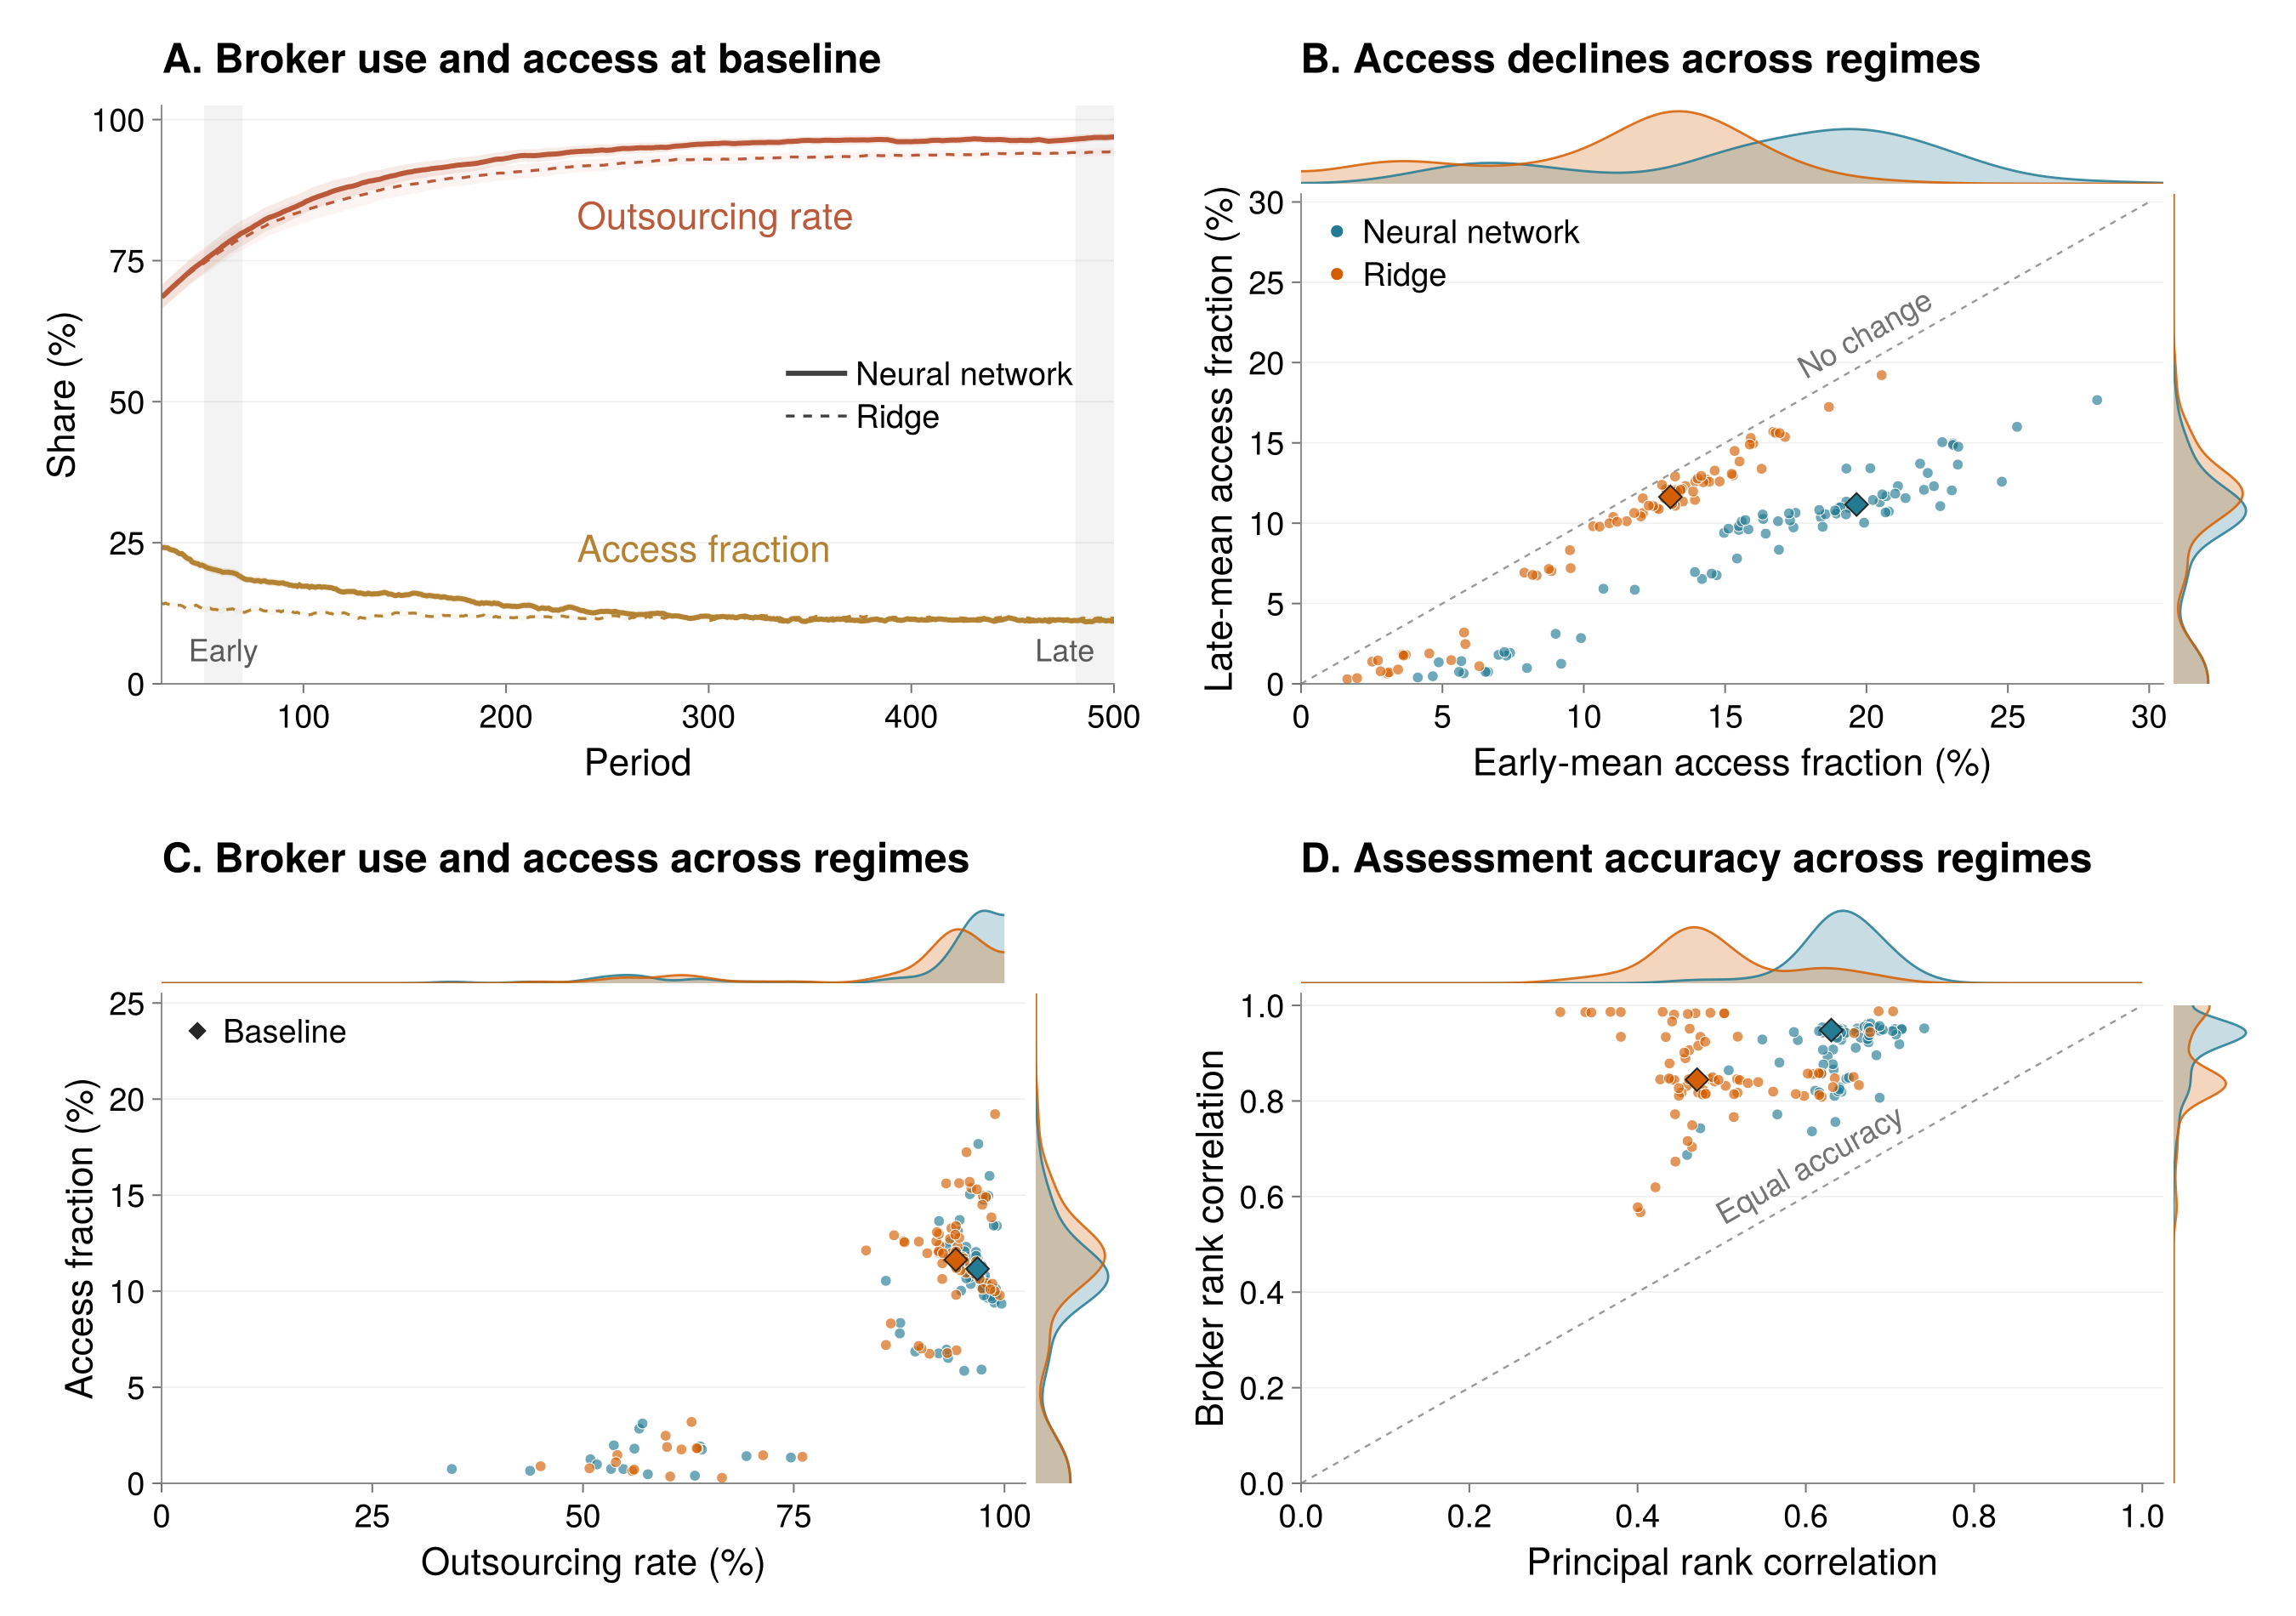
\includegraphics[width=\linewidth]{figures/assessment_not_access.png}
\caption{\textbf{Broker use, access, and assessment accuracy.} A: ensemble means after a 5-observation rolling mean within each seed, with pointwise 95\% Monte Carlo intervals. B--D: ensemble means for 80 regimes; C--D use late means. Marginal curves show smoothed distributions of regime means, with equal weight per regime and common smoothing across learners.}
\label{fig:dynamics}
\end{figure}

Assessment guides the broker's selection of counterparties: its predictions of match output determine how candidates are ranked and which offers are made first. The ranking diagnostic evaluates this component of the service by comparing the broker's and principals' predicted rankings against rankings by true expected match output on the same randomly sampled candidates. At baseline, late-mean rank correlation is 0.95 for the broker and 0.63 for principals, with a paired 95\% interval of [0.31, 0.33] for the ranking advantage. That advantage is positive in every regime, with all paired intervals above zero (Figure~\ref{fig:dynamics}, Panel~D).

The predominance of assessment compared to access also persists when the broker and the principals use Ridge regression to make their predictions instead of neural-network learning. In the Ridge variant, late-mean outsourcing exceeds one-half in 79 of 80 regimes, and the late-mean share of brokered placements reusing existing ties exceeds 80\% in every regime (Figure~\ref{fig:dynamics}, Panel~C). Neural-network learning raises principals' late-mean ranking accuracy in all 80 regimes and narrows the broker's ranking advantage in 64 (Panel~D), yet extensive outsourcing and the predominance of assessment persist.

Together, these findings identify assessment rather than new access as the broker's predominant service. Principals outsource the evaluation and arrangement of matches even when the counterparties involved are already reachable.

\subsection{The Value and Structural Consequences of Access and Assessment}
\label{sec:assessment-access}

The broker ranks candidates more accurately than principals, but ranking accuracy alone does not establish how much its assessments contribute to principals' net output. The assessment and access experiment examines these contributions by comparing full service with assessment-only and access-only service across 11 regimes varying turnover and matching composition. Each simulation uses one version of the broker's service throughout. Changing that service affects which principals match, how much demand they route through the broker, which ties form among principals and with the broker, and what principals and the broker subsequently learn.

\subsubsection{The Broker Can Benefit Principals by Providing Access While Eroding Its Structural Advantage}

A broker can increase principals' net output by providing access to counterparties beyond those available through ordinary self-search, even when most of its placements reuse existing ties. At baseline, principals' late-mean net output is 1.02 higher per principal under full service than under assessment-only service, with a paired 95\% interval of [0.96, 1.08] (Figure~\ref{fig:assessment-access}, Panel~A). Principals therefore benefit when the broker provides broader access alongside its assessments, even though only a minority of its placements connect previously unconnected principals.

\begin{figure}
\centering
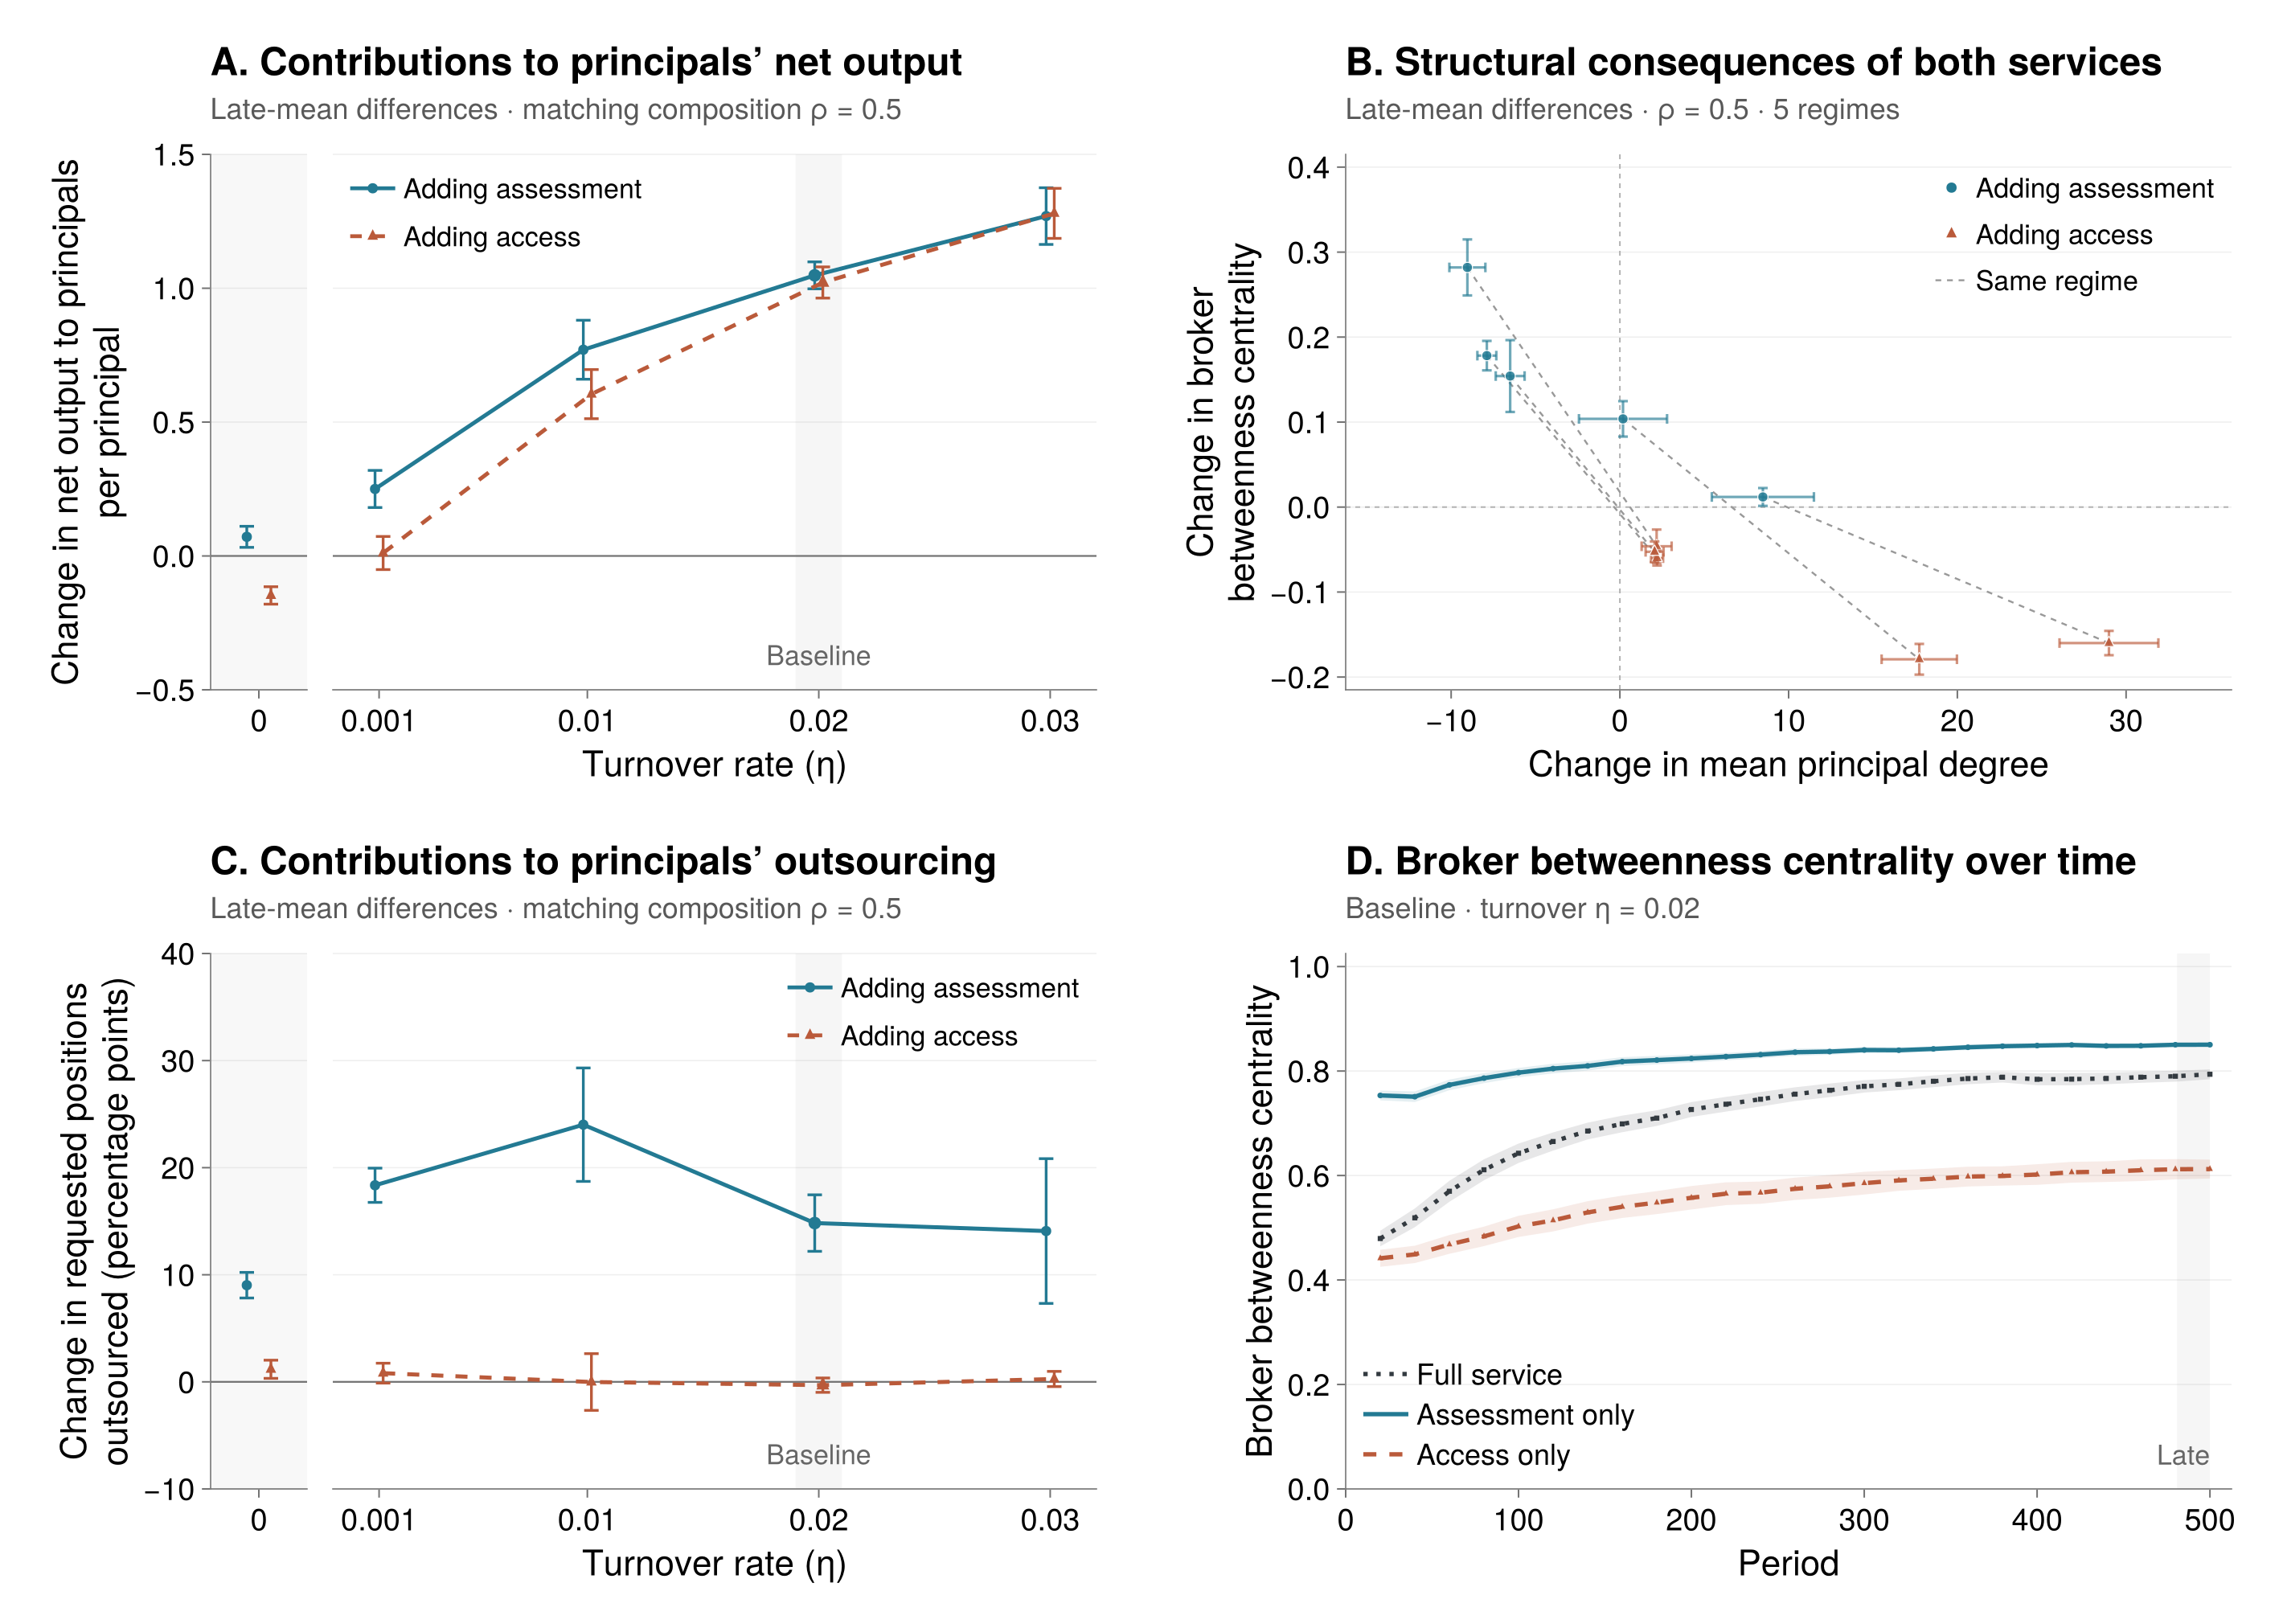
\includegraphics[width=\linewidth]{figures/assessment_access_3.png}
\caption{\textbf{Brokerage with access, assessment, or both.} Parameters other than turnover remain at baseline. A--C show late-mean differences: adding assessment is full service minus access-only; adding access is full service minus assessment-only. In B, dashed lines connect contrasts within each regime; principal degree includes the broker tie when present. Zero turnover is plotted separately in A and C. D shows unsmoothed ensemble means. Bars and ribbons show pointwise 95\% Monte Carlo intervals, paired by seed in A--C.}
\label{fig:assessment-access}
\end{figure}

This benefit depends on how frequently principals need new relationships. When 1\% or 3\% of participants leave and are replaced each period, principals obtain higher net output under full service than under assessment-only service across all matching compositions. Without turnover, principals obtain less net output under full service than under assessment-only service (Supplementary Figure~S4, Panel~B). Turnover continually removes principals and their relationships, making the broker's broader contacts useful for finding new counterparties. In stable markets, accumulated relationships and ordinary self-search already provide a viable candidate pool, so the broker does not necessarily improve principals' net output by reaching additional candidates.

The relative contributions of assessment and access also depend on principals' need for new relationships. Under pure complementarity and no turnover, principals' late-mean net output is 0.26 higher per principal under assessment-only than under access-only service, with a paired 95\% interval of [0.22, 0.30]. When 3\% of participants leave and are replaced each period, principals' late-mean net output is 0.22 higher per principal under access-only than under assessment-only service, with a paired 95\% interval of [0.13, 0.32] (Supplementary Figure~S4, Panels~A--B).

Comparing full service with assessment-only service also reveals a structural cost for the broker. At baseline, principals have more network ties on average under full service than under assessment-only service: their late-mean degree is 17.73 rather than 15.52. Degree counts each principal's ties to other principals and its tie to the broker when present. Meanwhile, the broker has lower late-mean betweenness centrality, 0.79 rather than 0.85 (Figure~\ref{fig:assessment-access}, Panel~B). Both directions hold in all 11 regimes, with paired 95\% intervals supporting each difference.

Providing assessment has the opposite effect on the broker's betweenness centrality. At baseline matching composition ($\rho=0.5$), the broker has higher late-mean betweenness centrality under full service than under access-only service at every turnover rate, with all paired 95\% intervals above zero (Panel~B).

When the broker arranges a match between previously unconnected principals, they acquire a direct tie. By helping principals form these relationships, the broker erodes the betweenness centrality it would otherwise accumulate. This is a self-liquidating force, not an inevitable absolute decline. At baseline, the broker's betweenness centrality rises even under access-only service, because principals' continued outsourcing still connects them to the broker (Figure~\ref{fig:assessment-access}, Panel~D).

\subsubsection{The Broker Can Sustain Demand Through Assessment Without Providing Additional Access}

The broker's assessments contribute to principals' net output alongside its broader contacts. At baseline, principals' late-mean net output is 1.05 higher per principal under full service than under access-only service, with a paired 95\% interval of [1.00, 1.10], compared with a gain of 1.02 over assessment-only service (Figure~\ref{fig:assessment-access}, Panel~A).

Principals continue to request brokerage even when the broker evaluates only candidates available through ordinary self-search. At baseline, late-mean outsourcing is 97\% under assessment-only service, compared with 97\% under full service and 82\% under access-only service. Principals outsource more when the broker uses its own assessments rather than theirs in every regime, with all paired intervals above zero. When the broker adds access to assessment-only service, principals make smaller changes in the share of requests they outsource, increasing it in some regimes and decreasing it in others (Figure~\ref{fig:assessment-access}, Panel~C).

These choices depend on principals' satisfaction with brokerage relative to self-search, based on the returns on their past matching requests after costs. Principals can therefore continue using the broker because their satisfaction with its service is high, because their satisfaction with self-search is low, or because both are true. Continued outsourcing establishes the broker's relative attractiveness, while the net-output comparisons establish the contribution of its assessments to principals' returns.

The assessment-only result also connects the ABM to data enclosure. The broker continues to create value for principals when it only assesses candidates they could reach through ordinary self-search. Its knowledge is therefore valuable independently of broader access. The experiment does not model data enclosure itself, because the broker still mediates matches and learns from them, but it establishes its prerequisite: assessment can become a distinct service that could be unbundled from intermediation and sold as predictions or analytics.

\subsection{The Broker's Information Advantage Comes from Data Volume and Relational Information}

The broker learns from the matches it arranges across principals, whereas each principal learns only from its own matches. This difference can support an assessment advantage in two ways: the broker has more observations, and it can learn how different parties' characteristics combine to produce match output. Three experiments distinguish these sources by reducing either the broker's training sample or the information it uses about each pairing.

All three experiments use Ridge regression for principals and the broker. The reference broker retains data about both parties to each brokered match and learns how their characteristics interact. Each restriction is compared with this reference across 31 regimes varying matching composition and difficulty.

Reducing the broker's training sample sharply narrows its advantage. The first restriction gives it as many observations as a typical principal, sampled from its records of brokered matches, with data about both parties retained. At baseline, its late-mean rank correlation falls from 0.84 in the reference version to 0.76, with a paired 95\% interval of [0.08, 0.10] for the decrease (Figure~\ref{fig:information-sources}, Panel~A). Its ranking advantage, the broker-minus-principal difference in rank correlation, falls from 0.37 to 0.04, with a paired 95\% interval of [0.32, 0.35] for the decrease. This larger change also reflects more accurate principal rankings: their late-mean rank correlation rises from 0.47 to 0.72.

\begin{figure}
\centering
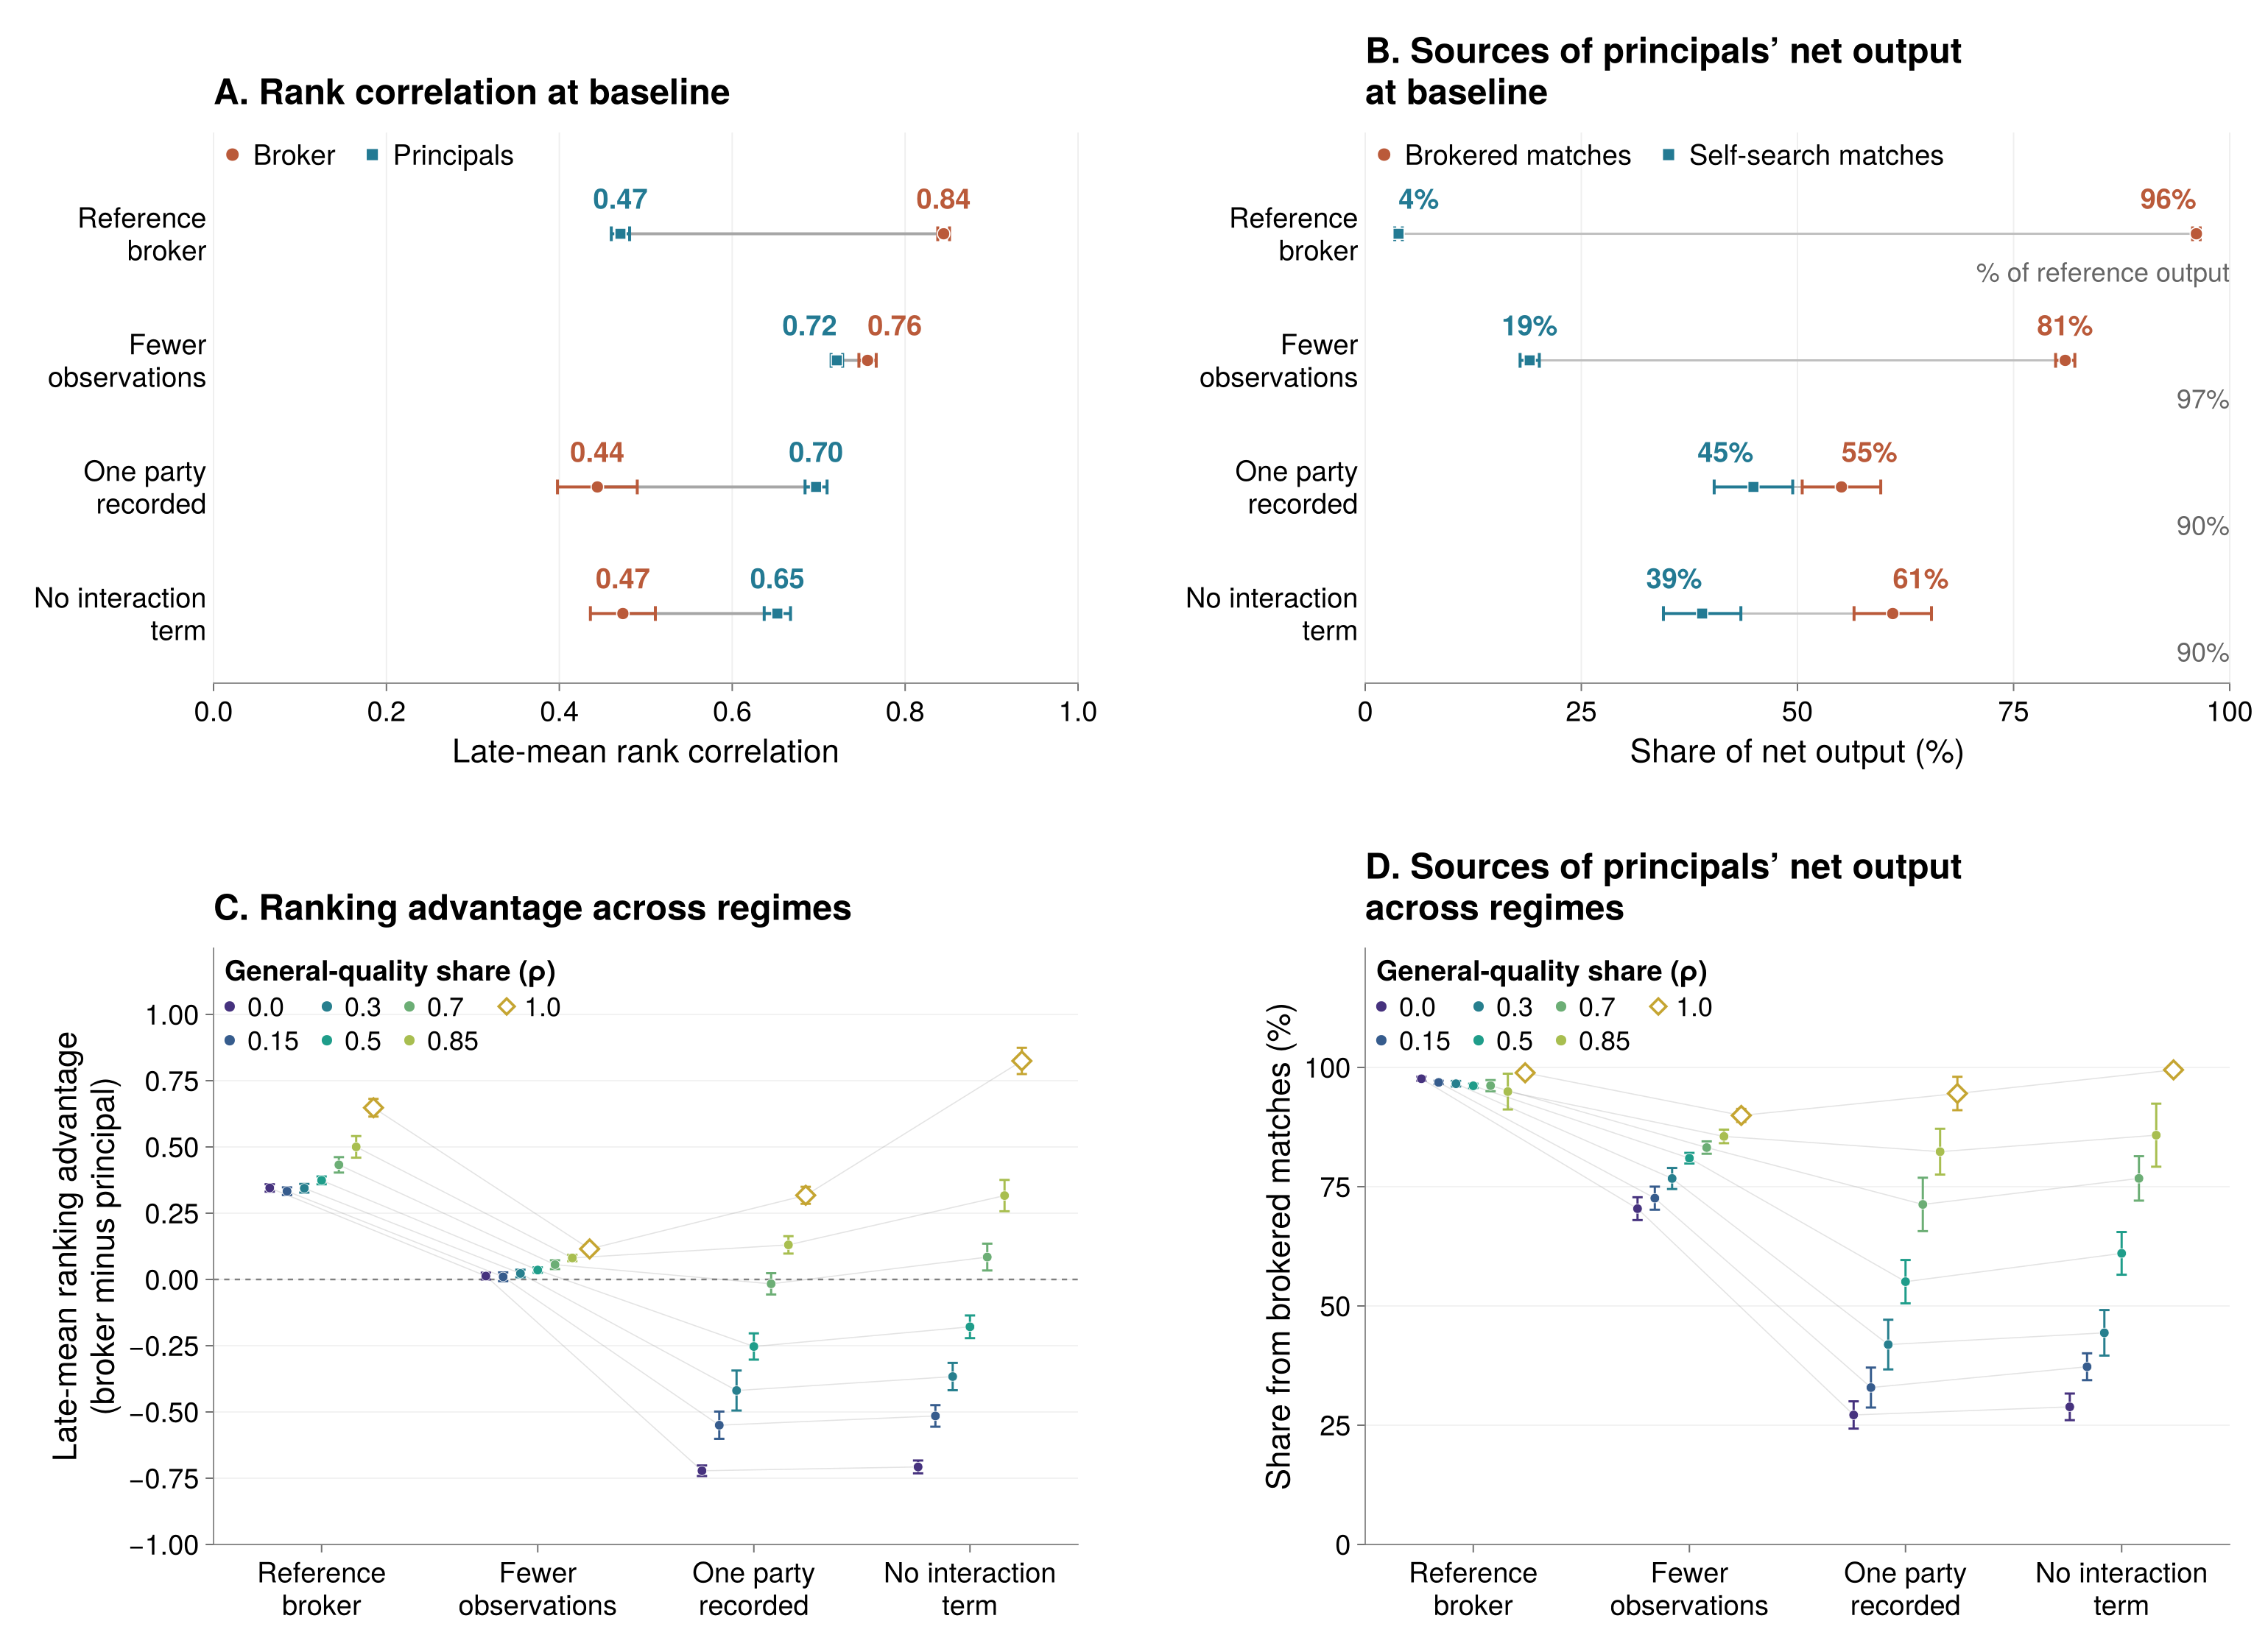
\includegraphics[width=\linewidth]{figures/information_sources_net_output_channels.png}
\caption{\textbf{Sources of the broker's advantage.} Ensemble late means from the Ridge experiments. Rank correlations use the same
randomly sampled candidates for principals and the broker. In C--D, parameters
other than $\rho$ remain at baseline; grey lines connect the same regime across
versions. Whiskers show pointwise 95\% Monte Carlo intervals.
C uses within-seed broker-minus-principal differences; B and D average seed-level
net-output shares. B's right-hand percentages compare ensemble-mean total net
output with the reference version.}
\label{fig:information-sources}
\end{figure}

Restricting the broker's learning throughout the simulation changes the matches it arranges and thus the observations from which principals learn. Both measures are lower than in the reference version in all 31 regimes, with paired intervals supporting every decrease, although a smaller ranking advantage persists in most. At baseline, the late-mean share of principals' net output from brokered matches falls from 96\% in the reference version to 81\%, while total net output is 97\% of reference output (Panel~B). Higher net output from self-search partially offsets lower net output from brokered matches.

Data volume does not explain the advantage by itself. Each principal's observations hold one party fixed: itself. The second broker restriction retains data about only one party to each match, alongside its realized output, while continuing to combine observations across principals. At baseline, the broker's late-mean rank correlation falls from 0.84 to 0.44, and its ranking advantage reverses from 0.37 to -0.25 (Panel~A). The 95\% interval for this broker-minus-principal difference is [-0.30, -0.20]. Both measures are lower than in the reference version in all 31 regimes, with paired intervals supporting every decrease. In 21 regimes, the interval for its ranking advantage lies entirely below zero. At baseline, the late-mean share of principals' net output from brokered matches falls from 96\% in the reference version to 55\%, and total net output is 90\% of reference output (Panel~B).

Retaining data about both parties also differs from learning how they combine. The third restriction omits the interaction term from the broker's predictions: it uses data about both parties, but one party's contribution cannot depend on the other's characteristics. At baseline, the broker's late-mean rank correlation falls from 0.84 to 0.47 and its ranking advantage from 0.37 to -0.18 (Panel~A). The paired 95\% interval for the 0.55 decrease in ranking advantage is [0.51, 0.60]. At baseline, the late-mean share of principals' net output from brokered matches falls from 96\% in the reference version to 61\%, and total net output is 90\% of reference output (Panel~B).

The broker's rank correlation is lower than in the reference version in all 30 regimes involving complementarity, with paired intervals supporting every decrease. Its ranking advantage also narrows in all 30, with paired intervals supporting 29 decreases. Under pure general quality, the restriction instead produces a higher broker rank correlation and a larger ranking advantage. Here, expected match output depends on the parties' separate contributions, rather than how their characteristics interact. Omitting the interaction term matches this simpler relationship and avoids estimating interactions that do not contribute to expected output.

These effects illustrate the importance of relational assessment. Removing data about one party or the interaction term reduces the broker's ranking advantage most under pure complementarity (Panel~C). At each difficulty level, these restrictions also shift a larger share of principals' net output from brokered matches toward self-search as complementarity contributes more to expected match output (Panel~D). Learning how particular parties fit together, beyond assessing their general quality, improves the broker's rankings and increases the share of principals' net output that comes from brokered matches.

Repeated vicarious relational work thus supplies both a larger sample and knowledge of which pairings succeed. Retaining data about both parties and learning how their characteristics combine make these observations useful for relational assessment.

\subsection{A Broker Can Be Highly Central While Doing Little Bridging}

The broker can become more central even as a smaller share of its placements connects previously unconnected principals. At baseline in the main simulations, broker betweenness centrality rises from an early mean of 0.55 to a late mean of 0.79, while the access fraction falls from 20\% to 11\%. A larger share of the shortest paths between principals therefore passes through the broker, even as its work becomes increasingly assessment-based. Such a central position is usually associated with connecting otherwise disconnected parties, yet a growing share of the broker's work takes place within relationships that already exist.

The broker's betweenness centrality depends on two kinds of ties: those connecting principals to the broker and those connecting principals to one another. Continued outsourcing connects principals to the broker. When the broker arranges matches within existing relationships, it sustains these connections without creating additional direct ties among principals. Providing access, by contrast, creates direct ties that offer alternative shortest paths bypassing the broker. These opposing effects appear in the assessment and access experiment: providing access lowers broker betweenness centrality, whereas providing assessment raises it (Figure~\ref{fig:assessment-access}, Panel~B).

Although brokerage is predominantly assessment-based across matching compositions, the broker's work becomes even more concentrated on assessment and its position in the network becomes more central as match output shifts from predominantly general quality to pure complementarity. At baseline turnover and difficulty, moving from $\rho=0.85$ to $\rho=0$ raises the late-mean share of brokered placements within existing relationships from 86\% to 90\% and broker betweenness centrality from 0.51 to 0.86 (Figure~\ref{fig:position}, Panel~A). Both differences occur at all 5 turnover rates, with paired 95\% intervals supporting each comparison.

\begin{figure}
\centering
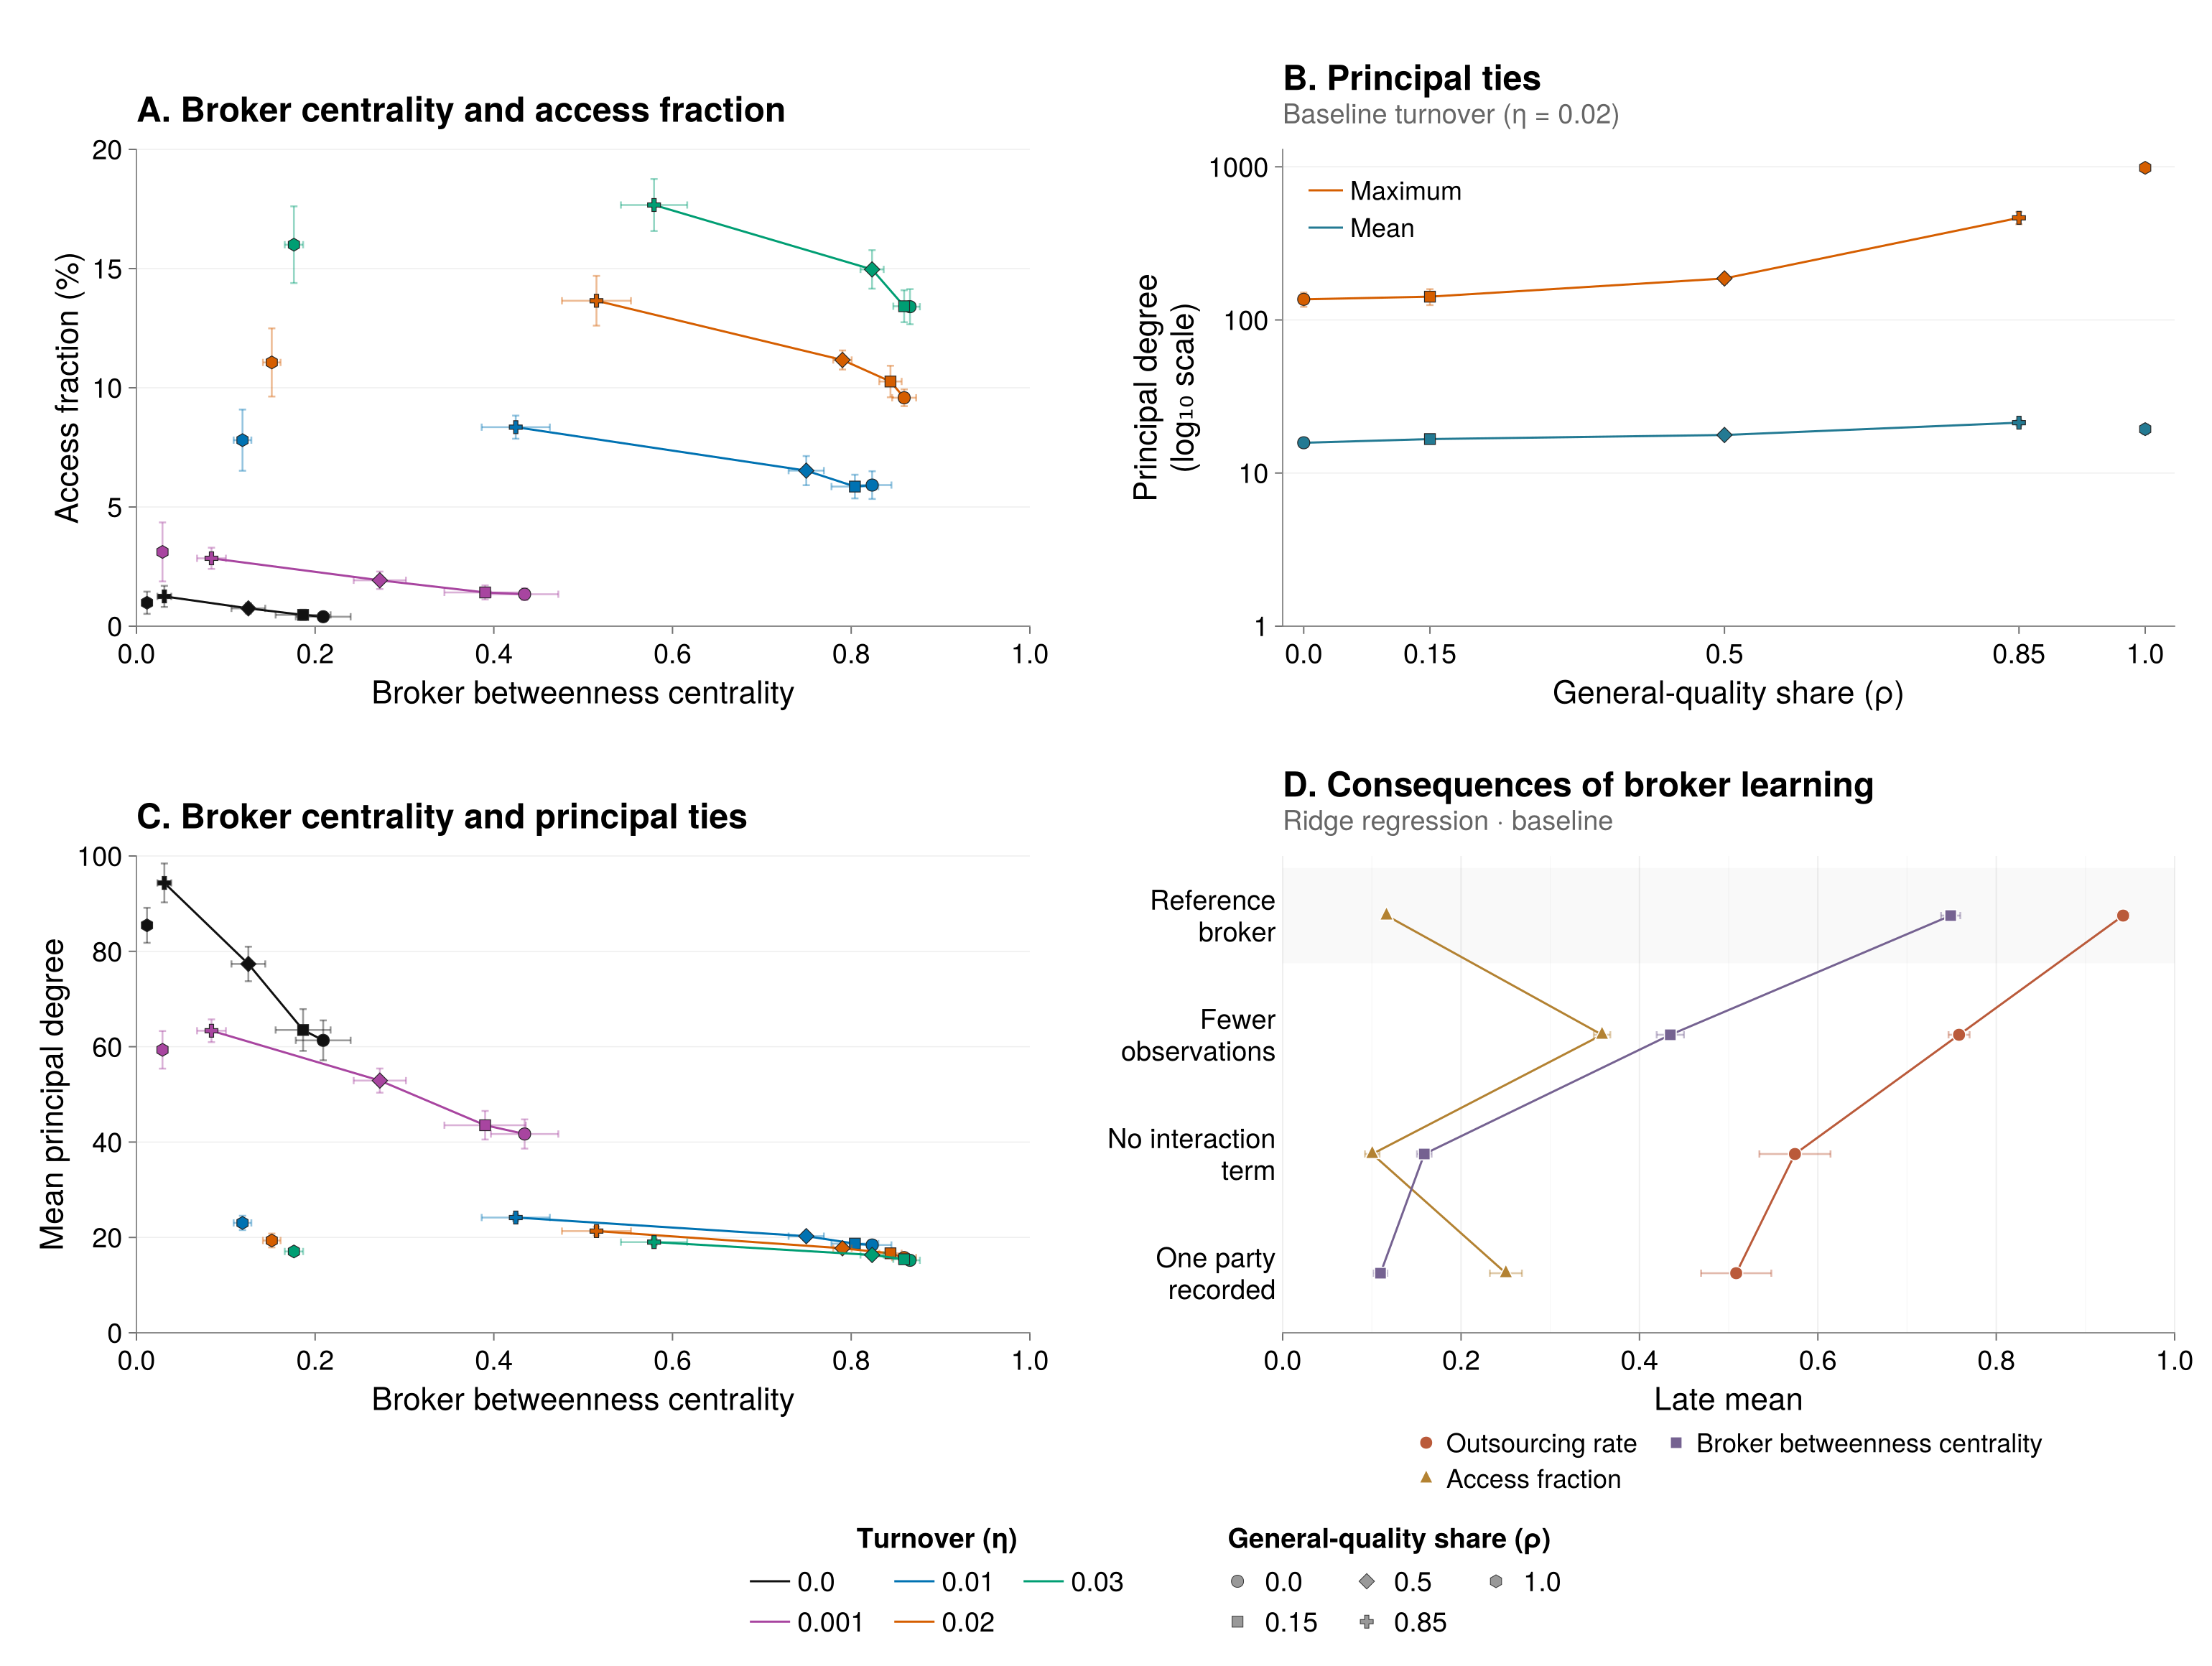
\includegraphics[width=\linewidth]{figures/centrality_and_assessment.png}
\caption{\textbf{Bridging position and bridging behavior.} Points show ensemble late means; whiskers show pointwise 95\% Monte Carlo intervals. A--C use neural-network learning; parameters not varied in each panel remain at baseline. Principal degree includes the broker tie when present; maximum degree is calculated within each period before averaging. Lines connect matching compositions at fixed turnover in A and C and serve as visual guides across learning restrictions in D.}
\label{fig:position}
\end{figure}

Extensive outsourcing and predominantly assessment-based brokerage do not by themselves ensure high broker betweenness centrality. The distribution of ties among principals also matters. When match output depends entirely on general quality ($\rho=1$), the baseline late-mean share of brokered placements within existing relationships is 89\% and outsourcing remains high at 97\%, but broker betweenness centrality is only 0.15. The same counterparties are attractive to many principals, allowing relationships to concentrate around them. The late mean of the maximum principal degree is 985.19, compared with 136.36 when output depends entirely on complementarity. Mean principal degree differs much less, at 19.36 and 15.77, respectively (Figure~\ref{fig:position}, Panel~B). A modest average degree can therefore conceal highly connected principals that provide alternative shortest paths that bypass the broker.

The persistence of principals' relationships also matters. Turnover continually removes principals and their ties, limiting the accumulation of paths that bypass the broker. At baseline matching composition and difficulty, replacing 3\% of principals each period rather than none lowers late-mean principal degree from 77.35 to 16.33 and raises broker betweenness centrality from 0.13 to 0.82 (Figure~\ref{fig:position}, Panel~C). The access fraction also rises, from 1\% to 15\% (Panel~A). A larger access fraction therefore does not necessarily imply lower broker betweenness centrality: newly formed ties can be offset by the loss of existing relationships.

The data and learning capabilities behind the broker's assessment advantage also help sustain its bridging position. At baseline in the Ridge experiment, omitting the interaction term reduces late-mean outsourcing from 94\% to 57\% and broker betweenness centrality from 0.75 to 0.16 (Figure~\ref{fig:position}, Panel~D). The late-mean access fraction remains low, at 10\% compared with 12\% for the reference broker. In both versions, most brokered placements reuse existing relationships, but the broker has much lower betweenness centrality when principals use its service less. Learning how parties fit together thus helps sustain principals' use of the broker and the connections that make it central.

Repeated vicarious relational work generates knowledge that can sustain principals' use of the broker. Sustained use converts the value of assessment into structural centrality, while the concentration and persistence of principals' own relationships shape how much centrality the broker attains. High broker betweenness centrality can therefore coexist with little bridging.

\subsection{Propositions}

The simulation results motivate the following falsifiable propositions for future empirical research:

\noindent\textbf{P1.} \textbf{\textit{When complementarity matters, assessment is the primary source of brokerage value}}. In matching markets that reward complementarity, brokers add value primarily by assessing counterparties rather than by bridging disconnected parties. The value of this assessment role increases as complementarity contributes more to match output.

\noindent\textbf{P2.} \textbf{\textit{Relationship disruption increases the value of access brokerage}}. Clients gain more from brokers' ability to find new counterparties when market participants frequently leave and are replaced than when they can rely on stable relationships.

\noindent\textbf{P3.} \textbf{\textit{When the broker records and accumulates data about his matching work, brokerage widens informational asymmetry}}. Repeated brokerage increases the broker's assessment advantage over his clients, even though those clients also learn from the matches he arranges.

\noindent\textbf{P4.} \textbf{\textit{Assessment brokerage produces high broker centrality with little bridging behavior}}. Sustained outsourcing converts the value of assessment into a greater structural centrality for the broker. Brokers whose assessments remain valuable relative to clients' independent alternatives become highly central even when most of their matches involve counterparties already connected to one another.

\noindent\textbf{P5.} \textbf{\textit{Assessment enables the broker to become a principal}}. Corporate brokers whose assessments create value independently of privileged access are more likely to use that capability on their own behalf, either to acquire and sell resources they previously intermediated (resource capture) or to sell predictions or analytics directly (data enclosure).
